% Se incluye el preambulo del trabajo
% Se configura el tipo de documento
\documentclass[a4paper]{article}

% Paquetes utilizados
\usepackage[utf8]{inputenc}
\usepackage[spanish, es-tabla]{babel}
\usepackage{float}
\usepackage{graphicx}
\usepackage{subcaption}

% Paquetes de matematica
\usepackage{amsmath}
\usepackage{steinmetz}

% Paquetes para excel
\usepackage{csvsimple}

% Configuracion del informe
\setlength{\parindent}{0pt}
\setcounter{secnumdepth}{0}

\usepackage[a4paper, 
    includehead, 
    footskip=7mm, 
    headsep=6mm, 
    headheight=4.8mm,
    top=25mm, bottom=25mm, left=25mm, right=25mm]{geometry}

%THIS IS FOR SETTING LOCATION OF FLOATS
\usepackage{float}
%ENDS SETTING LOCATION OF FLOATS

%THE FOLLOWING ARE CONFIGURATIONS FOR TODONOTES
\usepackage{todonotes,varwidth}
\makeatletter
\tikzstyle{diaanotestyle} = [
    draw=\@todonotes@currentbordercolor,
    fill=\@todonotes@currentbackgroundcolor,
    line width=0.5pt,
    inner sep = 0.8 ex,
    rounded corners=4pt,align=left,
   ]

\renewcommand{\@todonotes@drawInlineNote}{%
        {\begin{tikzpicture}[remember picture,baseline={(0,0)}]%
            \draw node[diaanotestyle,font=\@todonotes@sizecommand,anchor=base west]{%
               \begin{varwidth}[t]{10cm}
                \if@todonotes@authorgiven%
                    {\@todonotes@sizecommand \@todonotes@author:\,\@todonotes@text}%
                \else%
                    {\@todonotes@sizecommand \@todonotes@text}%
                \fi
                \end{varwidth}};%
            \end{tikzpicture}}%
       }%
\makeatother
%HERE ENDS THE CONFIGURATIONS FOR TODONOTES

%THIS IS FOR MERGING CELLS IN A TABLE
\usepackage{multirow}
%ENDS MERGING CELLS

\usepackage{hyperref}
\hypersetup{
    colorlinks=true,
    linkcolor=blue,
    filecolor=magenta,      
    urlcolor=blue,
    citecolor=blue,    
}

%MAPAS DE KARNAUGH
\usepackage{tikz}
\usetikzlibrary{matrix,calc}

%isolated term
%#1 - Optional. Space between node and grouping line. Default=0
%#2 - node
%#3 - filling color
\newcommand{\implicantsol}[3][0]{
    \draw[rounded corners=3pt, fill=#3, opacity=0.3] ($(#2.north west)+(135:#1)$) rectangle ($(#2.south east)+(-45:#1)$);
    }


%internal group
%#1 - Optional. Space between node and grouping line. Default=0
%#2 - top left node
%#3 - bottom right node
%#4 - filling color
\newcommand{\implicant}[4][0]{
    \draw[rounded corners=3pt, fill=#4, opacity=0.3] ($(#2.north west)+(135:#1)$) rectangle ($(#3.south east)+(-45:#1)$);
    }

%group lateral borders
%#1 - Optional. Space between node and grouping line. Default=0
%#2 - top left node
%#3 - bottom right node
%#4 - filling color
\newcommand{\implicantcostats}[4][0]{
    \draw[rounded corners=3pt, fill=#4, opacity=0.3] ($(rf.east |- #2.north)+(90:#1)$)-| ($(#2.east)+(0:#1)$) |- ($(rf.east |- #3.south)+(-90:#1)$);
    \draw[rounded corners=3pt, fill=#4, opacity=0.3] ($(cf.west |- #2.north)+(90:#1)$) -| ($(#3.west)+(180:#1)$) |- ($(cf.west |- #3.south)+(-90:#1)$);
}

%group top-bottom borders
%#1 - Optional. Space between node and grouping line. Default=0
%#2 - top left node
%#3 - bottom right node
%#4 - filling color
\newcommand{\implicantdaltbaix}[4][0]{
    \draw[rounded corners=3pt, fill=#4, opacity=0.3] ($(cf.south -| #2.west)+(180:#1)$) |- ($(#2.south)+(-90:#1)$) -| ($(cf.south -| #3.east)+(0:#1)$);
    \draw[rounded corners=3pt, fill=#4, opacity=0.3] ($(rf.north -| #2.west)+(180:#1)$) |- ($(#3.north)+(90:#1)$) -| ($(rf.north -| #3.east)+(0:#1)$);
}

%group corners
%#1 - Optional. Space between node and grouping line. Default=0
%#2 - filling color
\newcommand{\implicantcantons}[2][0]{
    \draw[rounded corners=3pt, opacity=.3] ($(rf.east |- 0.south)+(-90:#1)$) -| ($(0.east |- cf.south)+(0:#1)$);
    \draw[rounded corners=3pt, opacity=.3] ($(rf.east |- 8.north)+(90:#1)$) -| ($(8.east |- rf.north)+(0:#1)$);
    \draw[rounded corners=3pt, opacity=.3] ($(cf.west |- 2.south)+(-90:#1)$) -| ($(2.west |- cf.south)+(180:#1)$);
    \draw[rounded corners=3pt, opacity=.3] ($(cf.west |- 10.north)+(90:#1)$) -| ($(10.west |- rf.north)+(180:#1)$);
    \fill[rounded corners=3pt, fill=#2, opacity=.3] ($(rf.east |- 0.south)+(-90:#1)$) -|  ($(0.east |- cf.south)+(0:#1)$) [sharp corners] ($(rf.east |- 0.south)+(-90:#1)$) |-  ($(0.east |- cf.south)+(0:#1)$) ;
    \fill[rounded corners=3pt, fill=#2, opacity=.3] ($(rf.east |- 8.north)+(90:#1)$) -| ($(8.east |- rf.north)+(0:#1)$) [sharp corners] ($(rf.east |- 8.north)+(90:#1)$) |- ($(8.east |- rf.north)+(0:#1)$) ;
    \fill[rounded corners=3pt, fill=#2, opacity=.3] ($(cf.west |- 2.south)+(-90:#1)$) -| ($(2.west |- cf.south)+(180:#1)$) [sharp corners]($(cf.west |- 2.south)+(-90:#1)$) |- ($(2.west |- cf.south)+(180:#1)$) ;
    \fill[rounded corners=3pt, fill=#2, opacity=.3] ($(cf.west |- 10.north)+(90:#1)$) -| ($(10.west |- rf.north)+(180:#1)$) [sharp corners] ($(cf.west |- 10.north)+(90:#1)$) |- ($(10.west |- rf.north)+(180:#1)$) ;
}

%Empty Karnaugh map 4x4
\newenvironment{Karnaugh}%
{
\begin{tikzpicture}[baseline=(current bounding box.north),scale=0.8]
\draw (0,0) grid (4,4);
\draw (0,4) -- node [pos=0.7,above right,anchor=south west] {AB} node [pos=0.7,below left,anchor=north east] {CD} ++(135:1);
%
\matrix (mapa) [matrix of nodes,
        column sep={0.8cm,between origins},
        row sep={0.8cm,between origins},
        every node/.style={minimum size=0.3mm},
        anchor=8.center,
        ampersand replacement=\&] at (0.5,0.5)
{
                       \& |(c00)| 00         \& |(c01)| 01         \& |(c11)| 11         \& |(c10)| 10         \& |(cf)| \phantom{00} \\
|(r00)| 00             \& |(0)|  \phantom{0} \& |(1)|  \phantom{0} \& |(3)|  \phantom{0} \& |(2)|  \phantom{0} \&                     \\
|(r01)| 01             \& |(4)|  \phantom{0} \& |(5)|  \phantom{0} \& |(7)|  \phantom{0} \& |(6)|  \phantom{0} \&                     \\
|(r11)| 11             \& |(12)| \phantom{0} \& |(13)| \phantom{0} \& |(15)| \phantom{0} \& |(14)| \phantom{0} \&                     \\
|(r10)| 10             \& |(8)|  \phantom{0} \& |(9)|  \phantom{0} \& |(11)| \phantom{0} \& |(10)| \phantom{0} \&                     \\
|(rf) | \phantom{00}   \&                    \&                    \&                    \&                    \&                     \\
};
}%
{
\end{tikzpicture}
}

%Empty Karnaugh map 2x4
\newenvironment{Karnaughvuit}%
{
\begin{tikzpicture}[baseline=(current bounding box.north),scale=0.8]
\draw (0,0) grid (4,2);
\draw (0,2) -- node [pos=0.7,above right,anchor=south west] {BC} node [pos=0.7,below left,anchor=north east] {A} ++(135:1);
%
\matrix (mapa) [matrix of nodes,
        column sep={0.8cm,between origins},
        row sep={0.8cm,between origins},
        every node/.style={minimum size=0.3mm},
        anchor=4.center,
        ampersand replacement=\&] at (0.5,0.5)
{
                      \& |(c00)| 00         \& |(c01)| 01         \& |(c11)| 11         \& |(c10)| 10         \& |(cf)| \phantom{00} \\
|(r00)| 0             \& |(0)|  \phantom{0} \& |(1)|  \phantom{0} \& |(3)|  \phantom{0} \& |(2)|  \phantom{0} \&                     \\
|(r01)| 1             \& |(4)|  \phantom{0} \& |(5)|  \phantom{0} \& |(7)|  \phantom{0} \& |(6)|  \phantom{0} \&                     \\
|(rf) | \phantom{00}  \&                    \&                    \&                    \&                    \&                     \\
};
}%
{
\end{tikzpicture}
}

%Empty Karnaugh map 2x2
\newenvironment{Karnaughquatre}%
{
\begin{tikzpicture}[baseline=(current bounding box.north),scale=0.8]
\draw (0,0) grid (2,2);
\draw (0,2) -- node [pos=0.7,above right,anchor=south west] {b} node [pos=0.7,below left,anchor=north east] {a} ++(135:1);
%
\matrix (mapa) [matrix of nodes,
        column sep={0.8cm,between origins},
        row sep={0.8cm,between origins},
        every node/.style={minimum size=0.3mm},
        anchor=2.center,
        ampersand replacement=\&] at (0.5,0.5)
{
          \& |(c00)| 0          \& |(c01)| 1  \\
|(r00)| 0 \& |(0)|  \phantom{0} \& |(1)|  \phantom{0} \\
|(r01)| 1 \& |(2)|  \phantom{0} \& |(3)|  \phantom{0} \\
};
}%
{
\end{tikzpicture}
}

%Defines 8 or 16 values (0,1,X)
\newcommand{\contingut}[1]{%
\foreach \x [count=\xi from 0]  in {#1}
     \path (\xi) node {\x};
}

%Places 1 in listed positions
\newcommand{\minterms}[1]{%
    \foreach \x in {#1}
        \path (\x) node {1};
}

%Places 0 in listed positions
\newcommand{\maxterms}[1]{%
    \foreach \x in {#1}
        \path (\x) node {0};
}

%Places X in listed positions
\newcommand{\indeterminats}[1]{%
    \foreach \x in {#1}
        \path (\x) node {X};
}

% Se agrega el titulo o caratula del trabajo

% Se crea el documento y agregan los ejercicios
\begin{document}

	% Crear y configurar el titulo/caratula del informe
	\title{
		\normalfont \normalsize \textsc{Instituto Tecnol\'ogico de Buenos Aires} \\ [25pt]
		\huge Trabajo Pr\'actico N$^{\circ}$2 \\
		\author{
			\\Grupo 1:\\\\Farall, Facundo David\\Gaytan, Joaqu\'in Oscar\\Kammann, Lucas Agust\'in\\Maselli, Carlos Javier\\ \\ \\ \\
			Profesores: \\\\ Dewald, Kevin\\Wundes, Pablo\\Aguirre, Miguel \\ \\ 
		}
		\text{Electr\'onica III - 2019}
	}
	\pagenumbering{arabic}
	\maketitle
	\newpage

	% Se agrega el indice con el contenido del trabajo
	\tableofcontents

	\newpage
	\section{Tecnolog\'ias TTL, RTL, NMOS y CMOS}
La electr\'onica digital en sus bases dise\~na circuitos cuyo funcionamiento reproduce el sistema binario
y el algebra booleana que define las operaciones matem\'aticas entre las entidades que son los bits. Es de inter\'es estudiar los par\'ametros
que establecen los l\'imites f\'isicos al modelo conceptual de las compuertas l\'ogicas para diferentes tecnolog\'ias y topolog\'ias. Para esto, 
se dise\~na con diferentes tecnolog\'ias una compuerta NOT.
	\newpage
	\section{Ejercicio 2: Comparaci\'on de compuertas discretas con tecnolog\'ia TTL y CMOS}
Se plantea estudiar la compatibilidad de compuertas de tecnología TTL (a base de transistores BJT) con CMOS (transistores MOSFET), enfocando la problemática desde el 
estudio de sus características de márgen de ruido, y haciendo también mención al fanout. 
Se abordará este análisis mediante el estudio de caso de los integrados 74HC02, 74HCT02 y 74LS02, los cuales contienen 4 compuertas NOR cada uno, implementados mediante 
distintas tecnologías.



\subsection{Marco teórico}
Las letras LS en 74LS02 refieren "Low-power Schottky", una tecnología del tipo TTL que alcanza mejores rendimientos y velocidad gracias a la implementación de 
transistores Schottky, los cuales difieren de los clásicos BJT únicamente en el agregado de un diodo Schottky entre sus terminales Base y Colector.
Por otro lado, HC y HCT refieren a "High-speed CMOS", distinguiéndose HCT por ser compatible con las tecnologías TTL.

\begin{figure}[H]
    \centering
    \begin{tabular}{c c}
        
\includegraphics[width=0.1\textwidth]{../EJ2/Recursos/schottky_transistor_symbol} &
        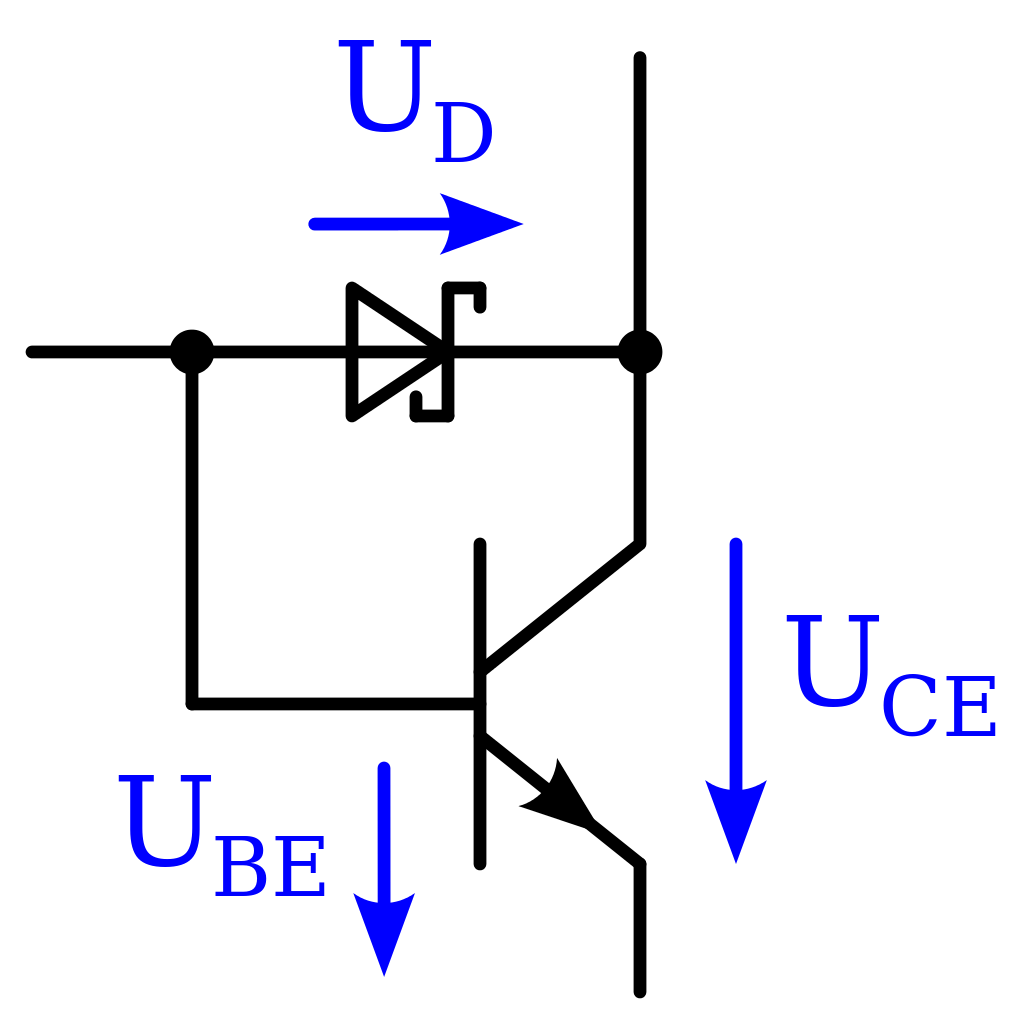
\includegraphics[width=0.1\textwidth]{../EJ2/Recursos/schottky_transistor_circuit}
    \end{tabular}
    \caption{Símbolo y circuito de transistor Schottky.}
    \label{fig:schottky_transistor_symbol_and_circuit_ex5}
\end{figure}

Tal y como fue mencionado en el inicio de esta sección, en este trabajo se estudiará la compatibilidad entre las tecnologías a través de sus márgenes de ruido.
Esto significa que, en términos de interconexión, una compuerta solo será compatible con otra de otra tecnología, si el rango de valores de salida de la primera está 
incluido en el rango de entrada de la segunda. \\
En las figuras \ref{fig:compatible_v_non_compatible_ex5} y \ref{fig:compatible_v_non_compatible_2_ex5} pueden apreciarse los casos que pueden presentarse que significarán la compatibilidad o no entre las compuertas.
De ellos se extrae que las compuertas serán compatibles solo en el caso en que $V_{OH} \geq V_{IH}$ y $V_{OL} \leq V_{IL}$.

\begin{figure}[H]
    \centering
    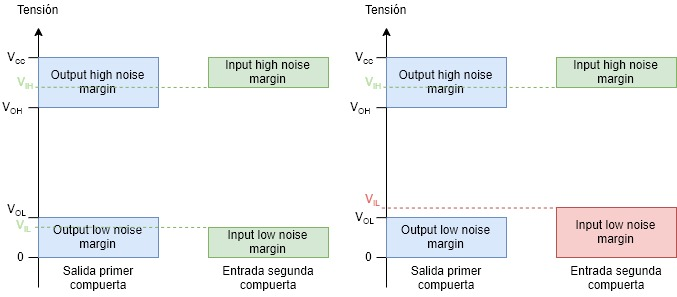
\includegraphics[width=0.9\textwidth]{../EJ2/Recursos/compatible_gates}
    \caption{Compatibilidad de compuertas.}
    \label{fig:compatible_v_non_compatible_ex5}
\end{figure}

\begin{figure}[H]
    \centering
    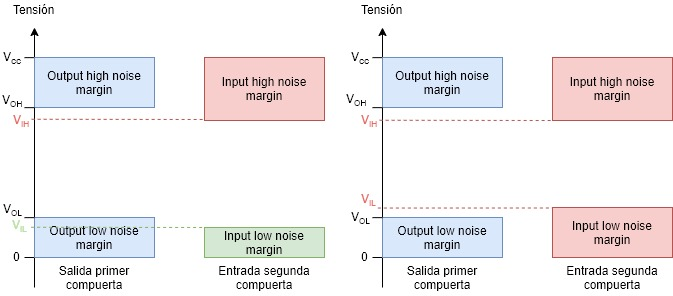
\includegraphics[width=0.9\textwidth]{../EJ2/Recursos/incompatible_gates}
    \caption{Compatibilidad de compuertas.}
    \label{fig:compatible_v_non_compatible_2_ex5}
\end{figure}

Con respecto al fanout, el mismo es una limitación para la cantidad de compuertas que se pueden colocar a la salida de otra, que viene dada por las corrientes de entrada 
y salida, respectivamente.

\begin{equation}
    fanout = min\left(\frac{I_{OH}}{I_{IH}} ; \frac{I_{OL}}{I_{IL}}\right)
\end{equation}



\subsection{Análisis mediante hojas de datos}
Se estudia la compatibilidad de la interconexión de las compuertas mediante la observación de las hojas de datos de los integrados 
74HC02\footnote{http://pdf.datasheetcatalog.com/datasheet/NXP\_Semiconductors/74HC\_HCT02.pdf}, 74HCT02\footnote{http://pdf.datasheetcatalog.com/datasheet/NXP\_Semiconductors/74HC\_HCT02.pdf} y 74LS02\footnote{http://www.sycelectronica.com.ar/semiconductores/74LS02.pdf},
y se exponen los datos utilizados en la tabla \ref{table:parameters_datasheet_ex5}.
Cabe mencionar que las condiciones de prueba de estos parámetros no son las mismas para las compuertas de tecnología CMOS que para las de TTL, de modo que se decide tomar 
el caso más desfavorable para cada una de las comparaciones.
En todos los casos, este terminó siendo que para las compuertas HC y HCT, la alimentación es de $4,5 V$, mientras que para las LS es de $5 V$.

\begin{table}[H]
    \begin{tabular}{ccccccccc}
    \textbf{Integrado} & \textbf{$V_{OH}$} & \textbf{$V_{OL}$} & \textbf{$V_{IH}$} & \textbf{$V_{IL}$} & \textbf{$I_{OH}$} & \textbf{$I_{OL}$} & \textbf{$I_{IH}$} & \textbf{$I_{IL}$} \\ \hline
    \textbf{74HC02}    & $4,4 V$           & $0,1 V$           & $3,15 V$          & $1,35 V$          & $\pm 25 mA$       & $\pm 25 mA$       & $\pm 0,1 \mu A$   & $\pm 0,1 \mu A$   \\
    \textbf{74HCT02}   & $4,4 V$           & $0,1 V$           & $2 V$             & $0,8 V$           & $\pm 25 mA$       & $\pm 25 mA$       & $\pm 0,1 \mu A$   & $\pm 0,1 \mu A$   \\
    \textbf{74LS02}    & $2,7 V$           & $0,5 V$           & $2 V$             & $0,8 V$           & $-0,4 mA$         & $8 mA$            & $20 \mu A$        & $-0,4 mA$        
    \end{tabular}
    \caption{Parámetros de compatibilidad obtenidos de datasheet.}
    \label{table:parameters_datasheet_ex5}
\end{table}

Se desprende de los datos expuestos y de la teoría explicada en el marco teórico, que son compatibles las conexiones de una compuerta HC a LS, de una HCT a LS, y de una 
LS a una HCT, ya que en todos estos casos se cumple que $V_{OH} \geq V_{IH}$ y $V_{OL} \leq V_{IL}$.
También es este el caso entre HCT y HC, y viceversa, resultado que es de esperar ya que comparten el tipo de tecnología.
Sin embargo, no sucede esto al ir de una LS a una HC ya que para esta combinación $V_{OH} < V_{IH}$, quedando una zona de indeterminación entre los valores de tensión 
$2,7 V$ y $3,15 V$.
Esta incompatibilidad es lógicamente salvada al usar tecnología HCT, la cual está diseñada con el propósito de lograr la compatibilidad que carecen las compuertas HC 
entre tecnologías TTL y CMOS.\\
En lo que respecta al fanout, los resultados son los expuestos en la tabla \ref{table:fanout_results_ex5}
\begin{table}[H]
    \begin{tabular}{ccccccc}
    \textbf{Interconexión} & \textbf{HC a LS} & \textbf{LS a HC} & \textbf{HCT a LS} & \textbf{LS a HCT} & \textbf{HC a HCT} & \textbf{HCT a HC} \\ \hline
    \textbf{fanout}        & $62$             & $4000$           & $62$              & $4000$            & $250 \cdot 10^3$  & $250 \cdot 10^3$ 
    \end{tabular}
    \caption{Fanout para distintas conexiones.}
    \label{table:fanout_results_ex5}
\end{table}



\subsection{Resultados experimentales}
Para el caso donde las hojas de datos no aseguran el correcto funcionamiento de la interconexión de compuertas, es decir, de una LS a una HC, se procede a estudiar su 
respuesta de forma experimental.
Se alimenta una compuerta del 74LS02 utilizada como NOT (cortocircuitando sus dos entradas) con una función rampa de 0 a 5V, y a su salida se conecta una del 74HC02, 
también como NOT. 
Se miden las salidas de ambas y los resultados son los expuestos en las figuras \ref{fig:LS_L_v_HC_H_ex5} y \ref{fig:LS_H_v_HC_L_ex5}.\\
Luego se realiza el mismo procedimiento pero en el lugar del 74HC02 se coloca el 74HCT02, cuyos resultados son los de las figuras \ref{fig:LS_L_v_HCT_H_ex5} y \ref{fig:LS_H_v_HCT_L_ex5}.
Se esperan observar indeterminaciones para la primer interconexión, y que tales problemas se vean resueltos al cambiar la tecnología HC por HCT. 

\begin{figure}[H]
    \centering
    \begin{tabular}{c c}
        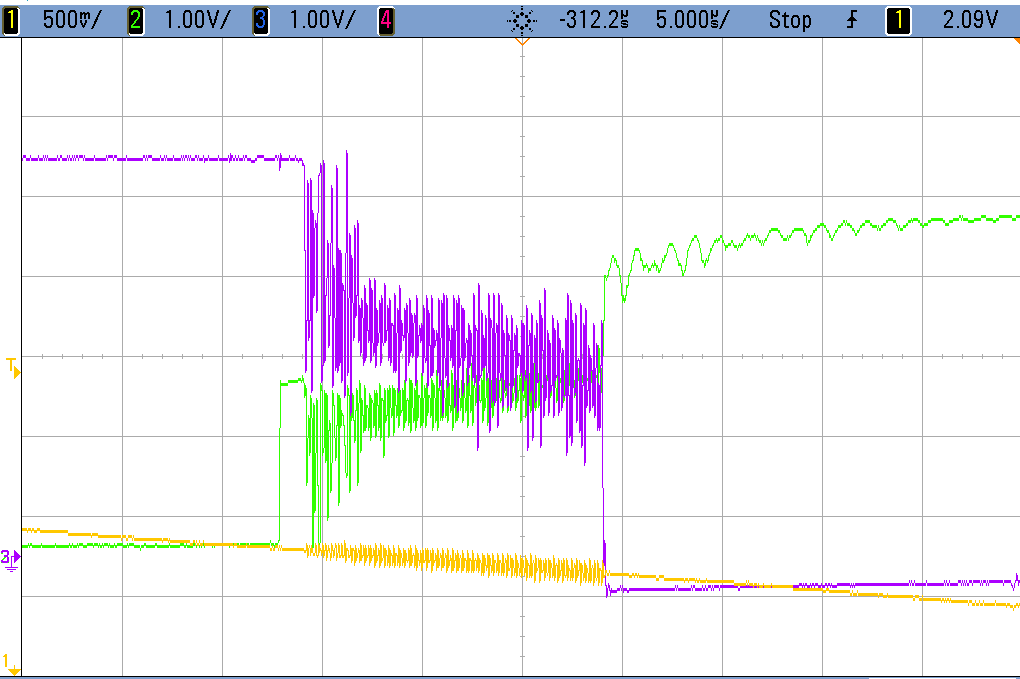
\includegraphics[width=0.5\textwidth]{../EJ2/Recursos/scope_32} &
        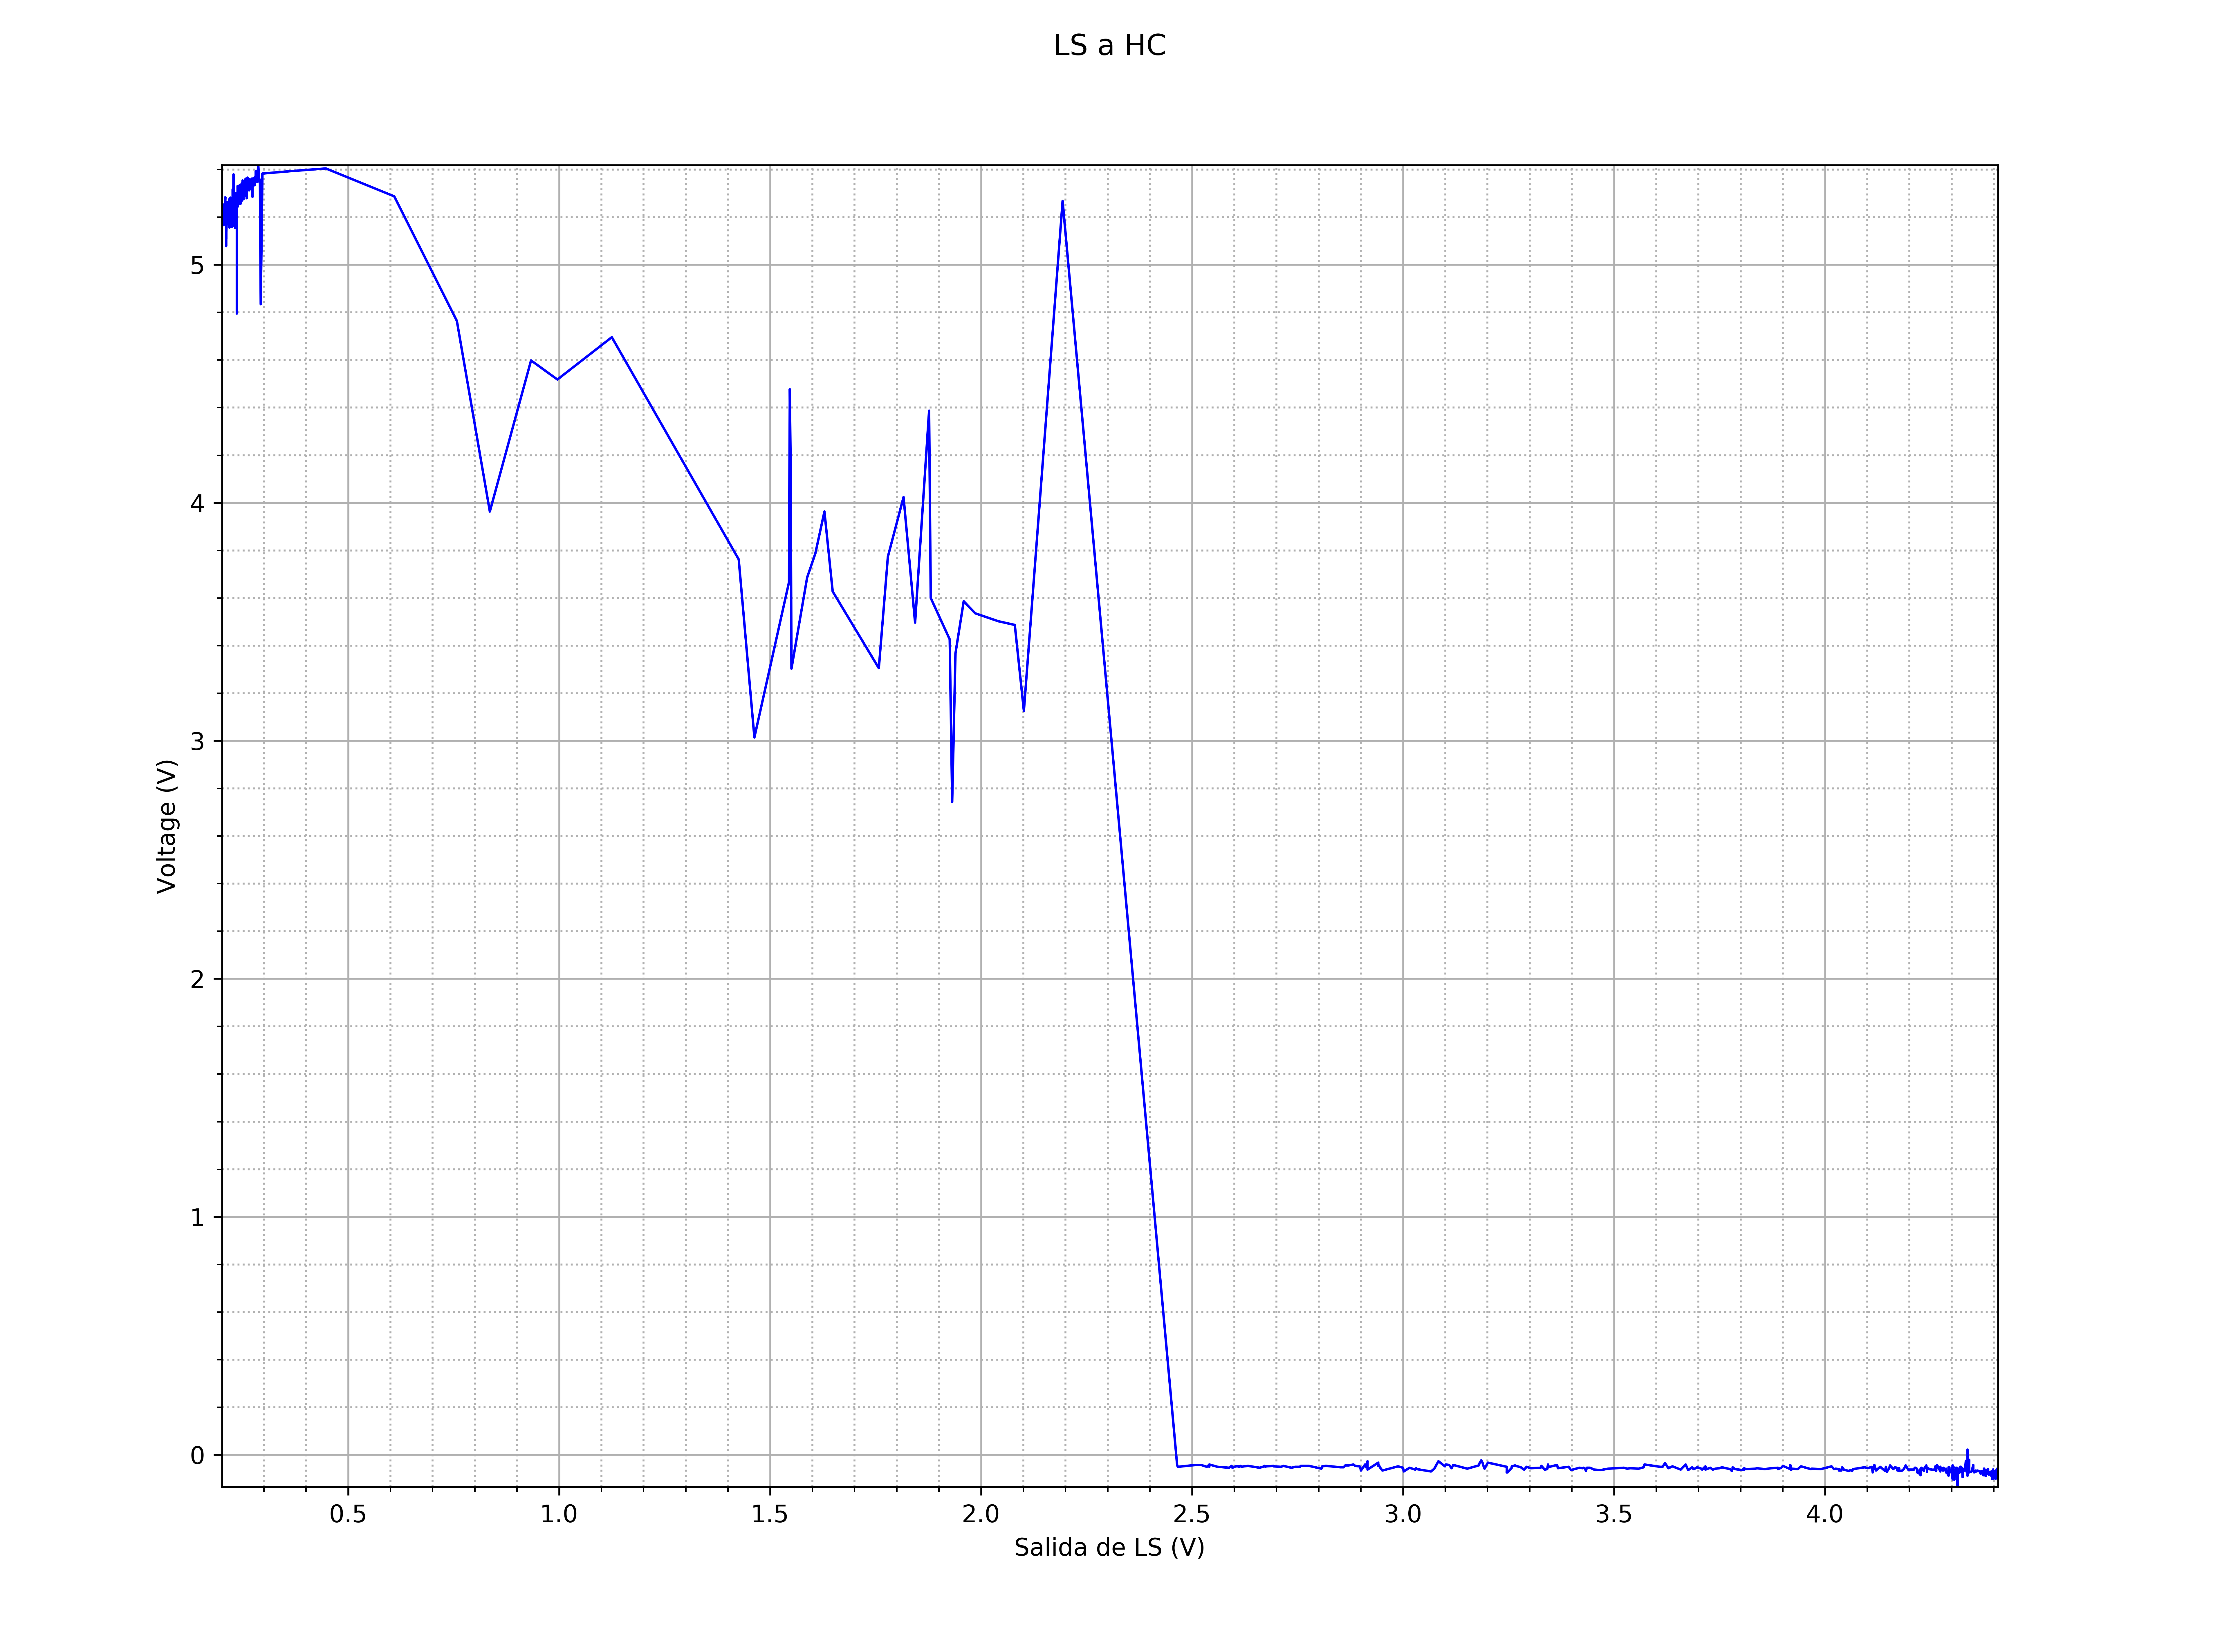
\includegraphics[width=0.5\textwidth]{../EJ2/Recursos/LS_L_v_HC_H}
    \end{tabular}
    \caption{LS a HC, con LS pasando de 0 a 1, y HC de 1 a 0.}
    \label{fig:LS_L_v_HC_H_ex5}
\end{figure}
\begin{figure}[H]
    \centering
    \begin{tabular}{c c}
        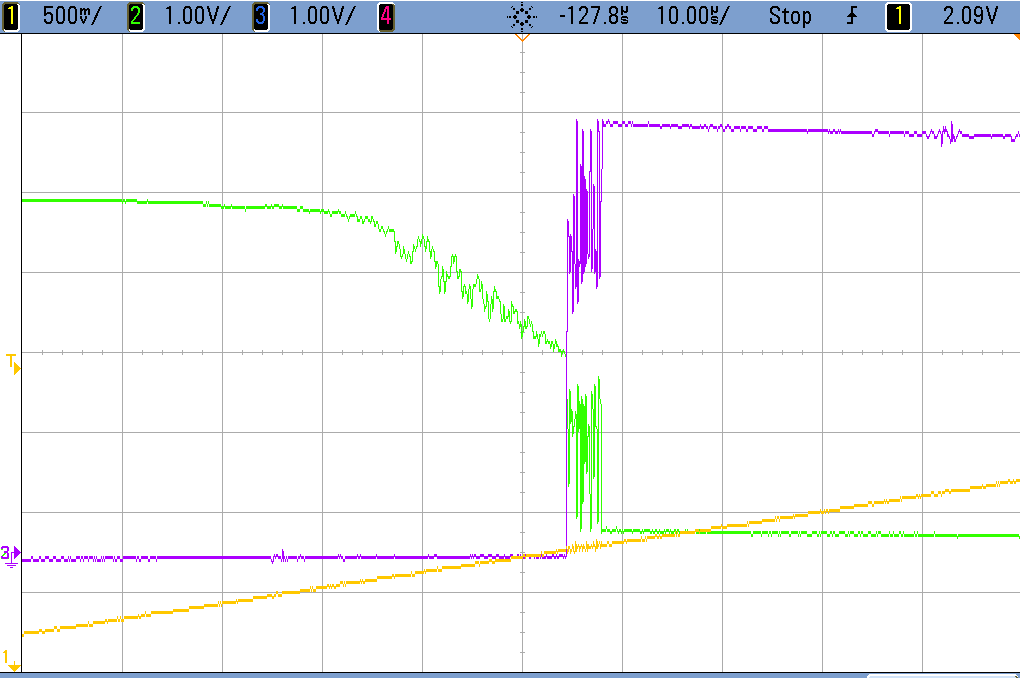
\includegraphics[width=0.5\textwidth]{../EJ2/Recursos/scope_29} &
        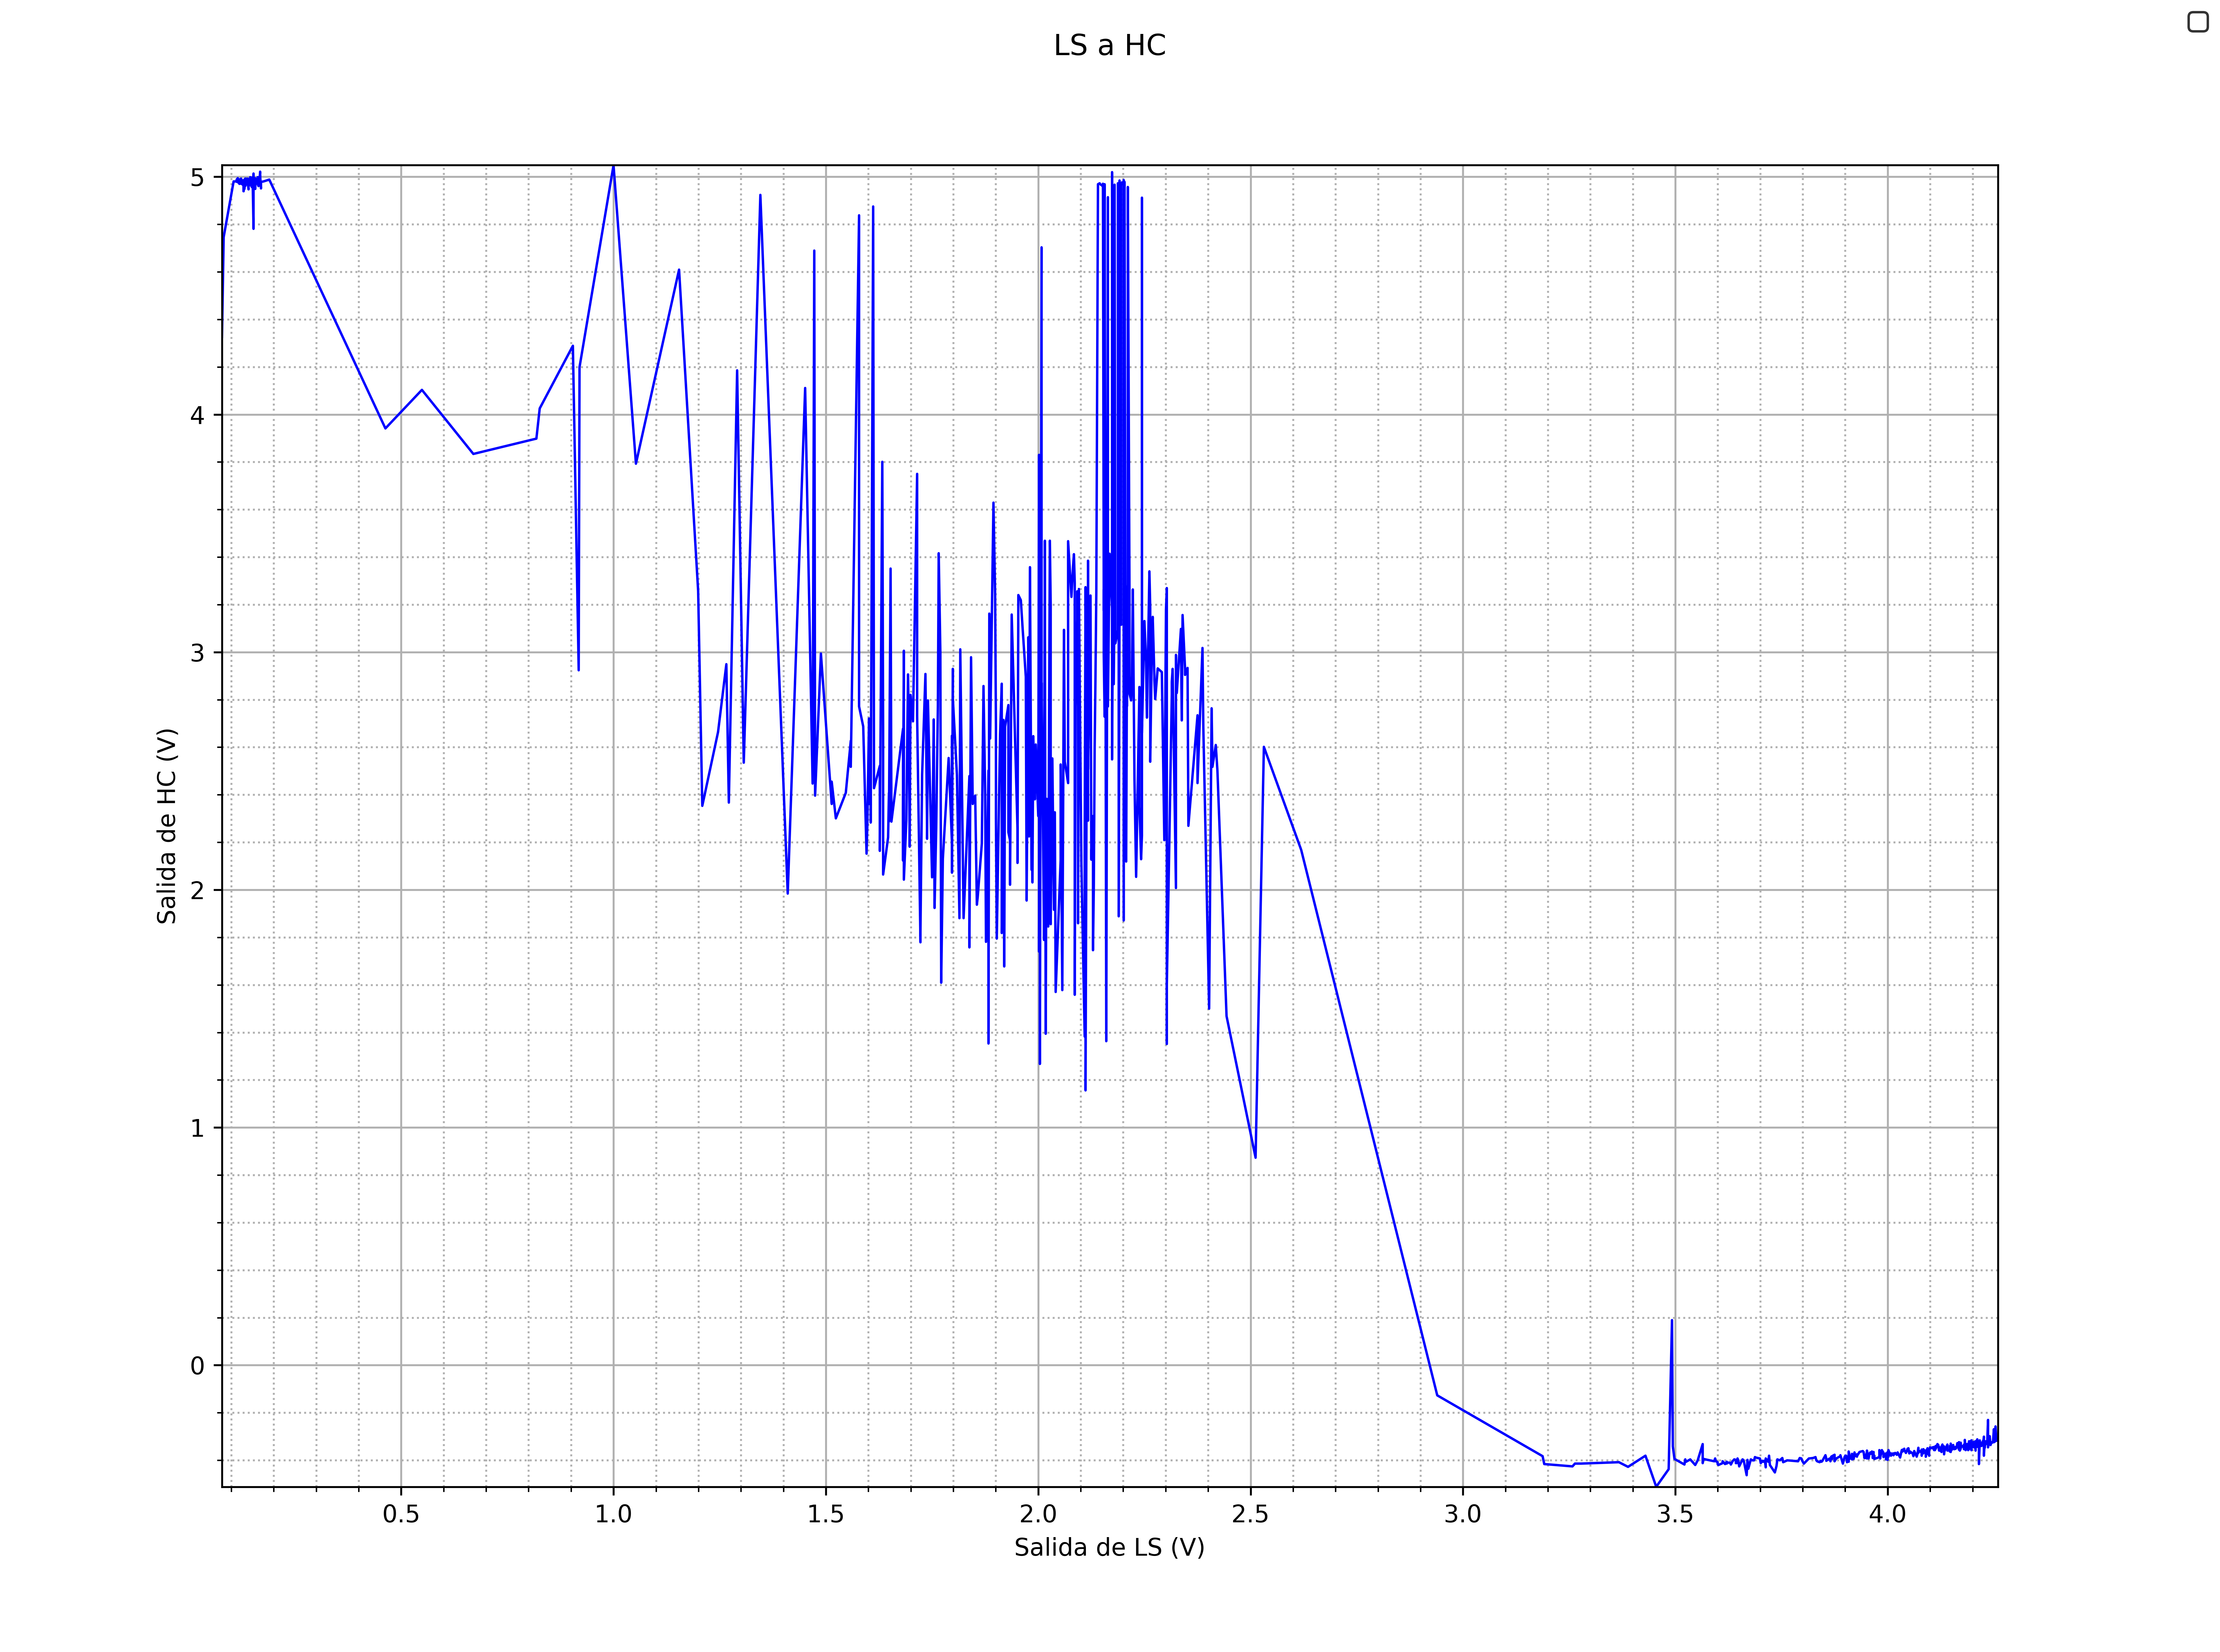
\includegraphics[width=0.5\textwidth]{../EJ2/Recursos/LS_H_v_HC_L}
    \end{tabular}
    \caption{LS a HC, con LS pasando de 1 a 0, y HC de 0 a 1.}
    \label{fig:LS_H_v_HC_L_ex5}
\end{figure}

\begin{figure}[H]
    \centering
    \begin{tabular}{c c}
        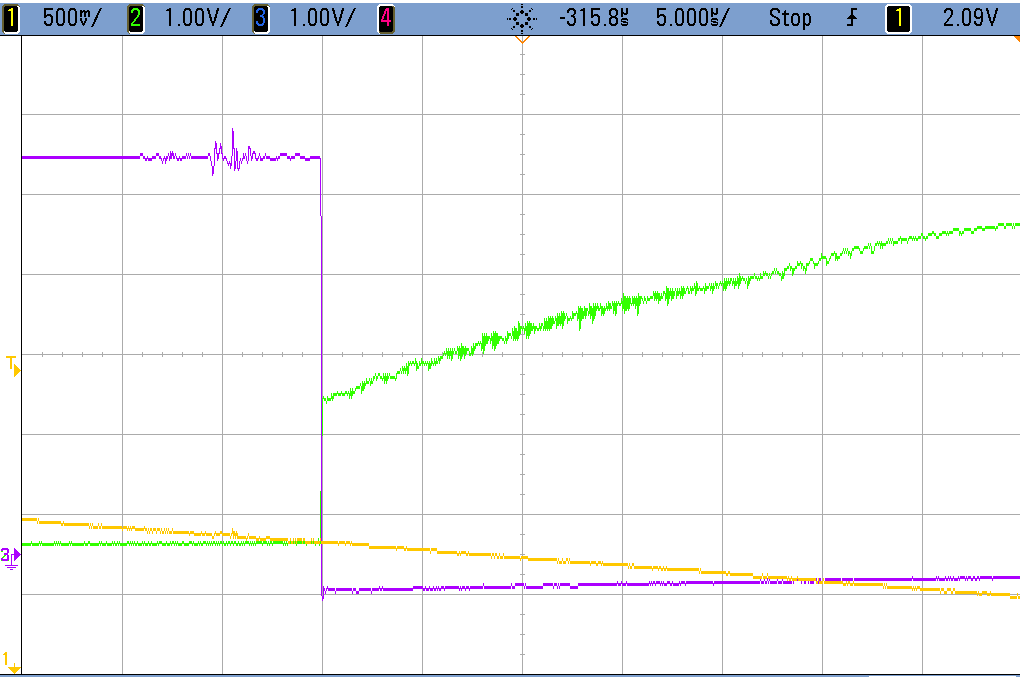
\includegraphics[width=0.5\textwidth]{../EJ2/Recursos/scope_38} &
        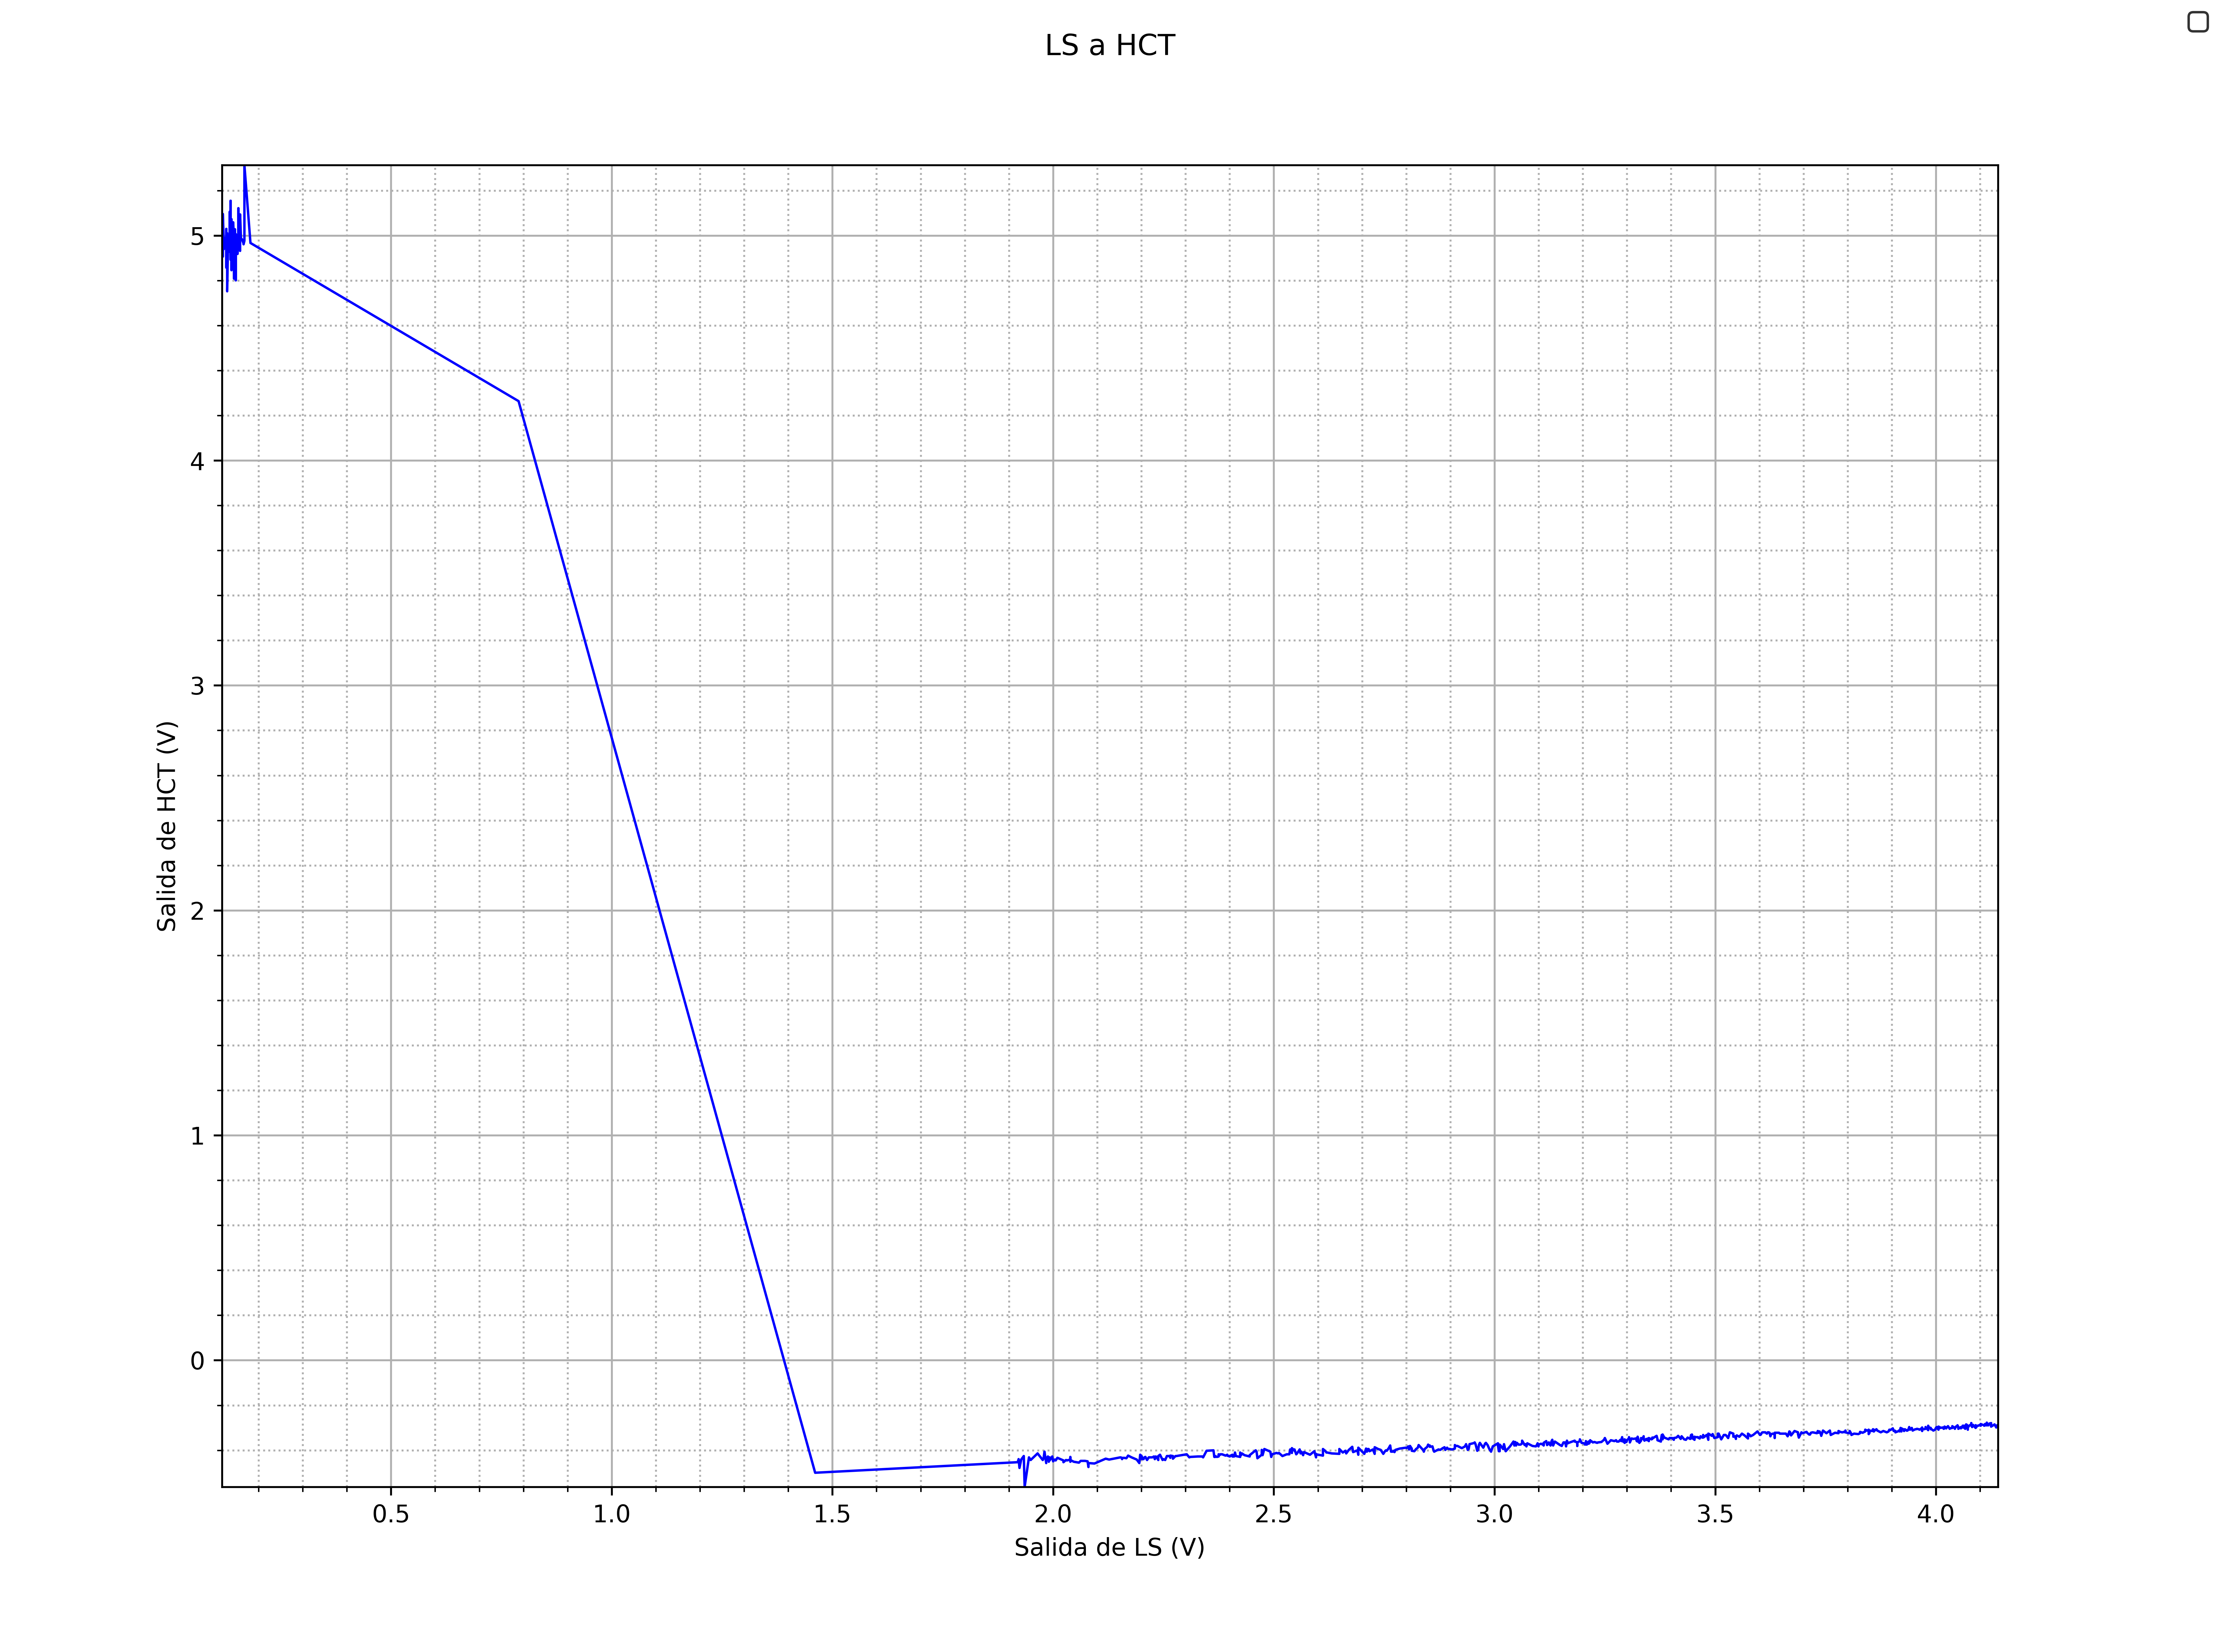
\includegraphics[width=0.5\textwidth]{../EJ2/Recursos/LS_L_v_HCT_H}
    \end{tabular}
    \caption{LS a HCT, con LS pasando de 0 a 1, y HCT de 1 a 0.}
    \label{fig:LS_L_v_HCT_H_ex5}
\end{figure}
\begin{figure}[H]
    \centering
    \begin{tabular}{c c}
        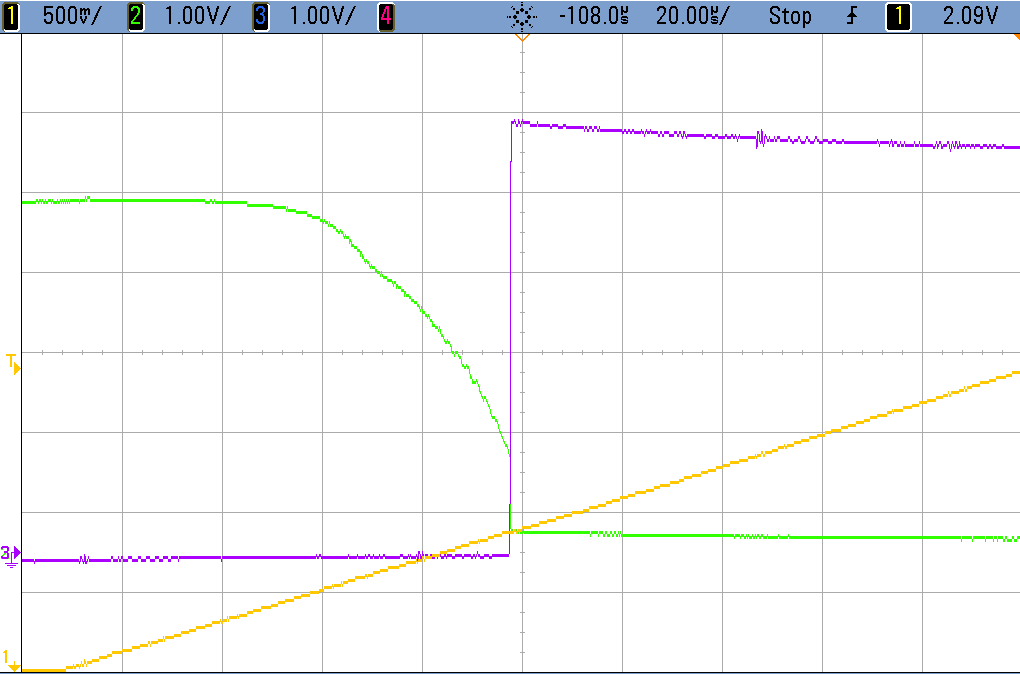
\includegraphics[width=0.5\textwidth]{../EJ2/Recursos/scope_35} &
        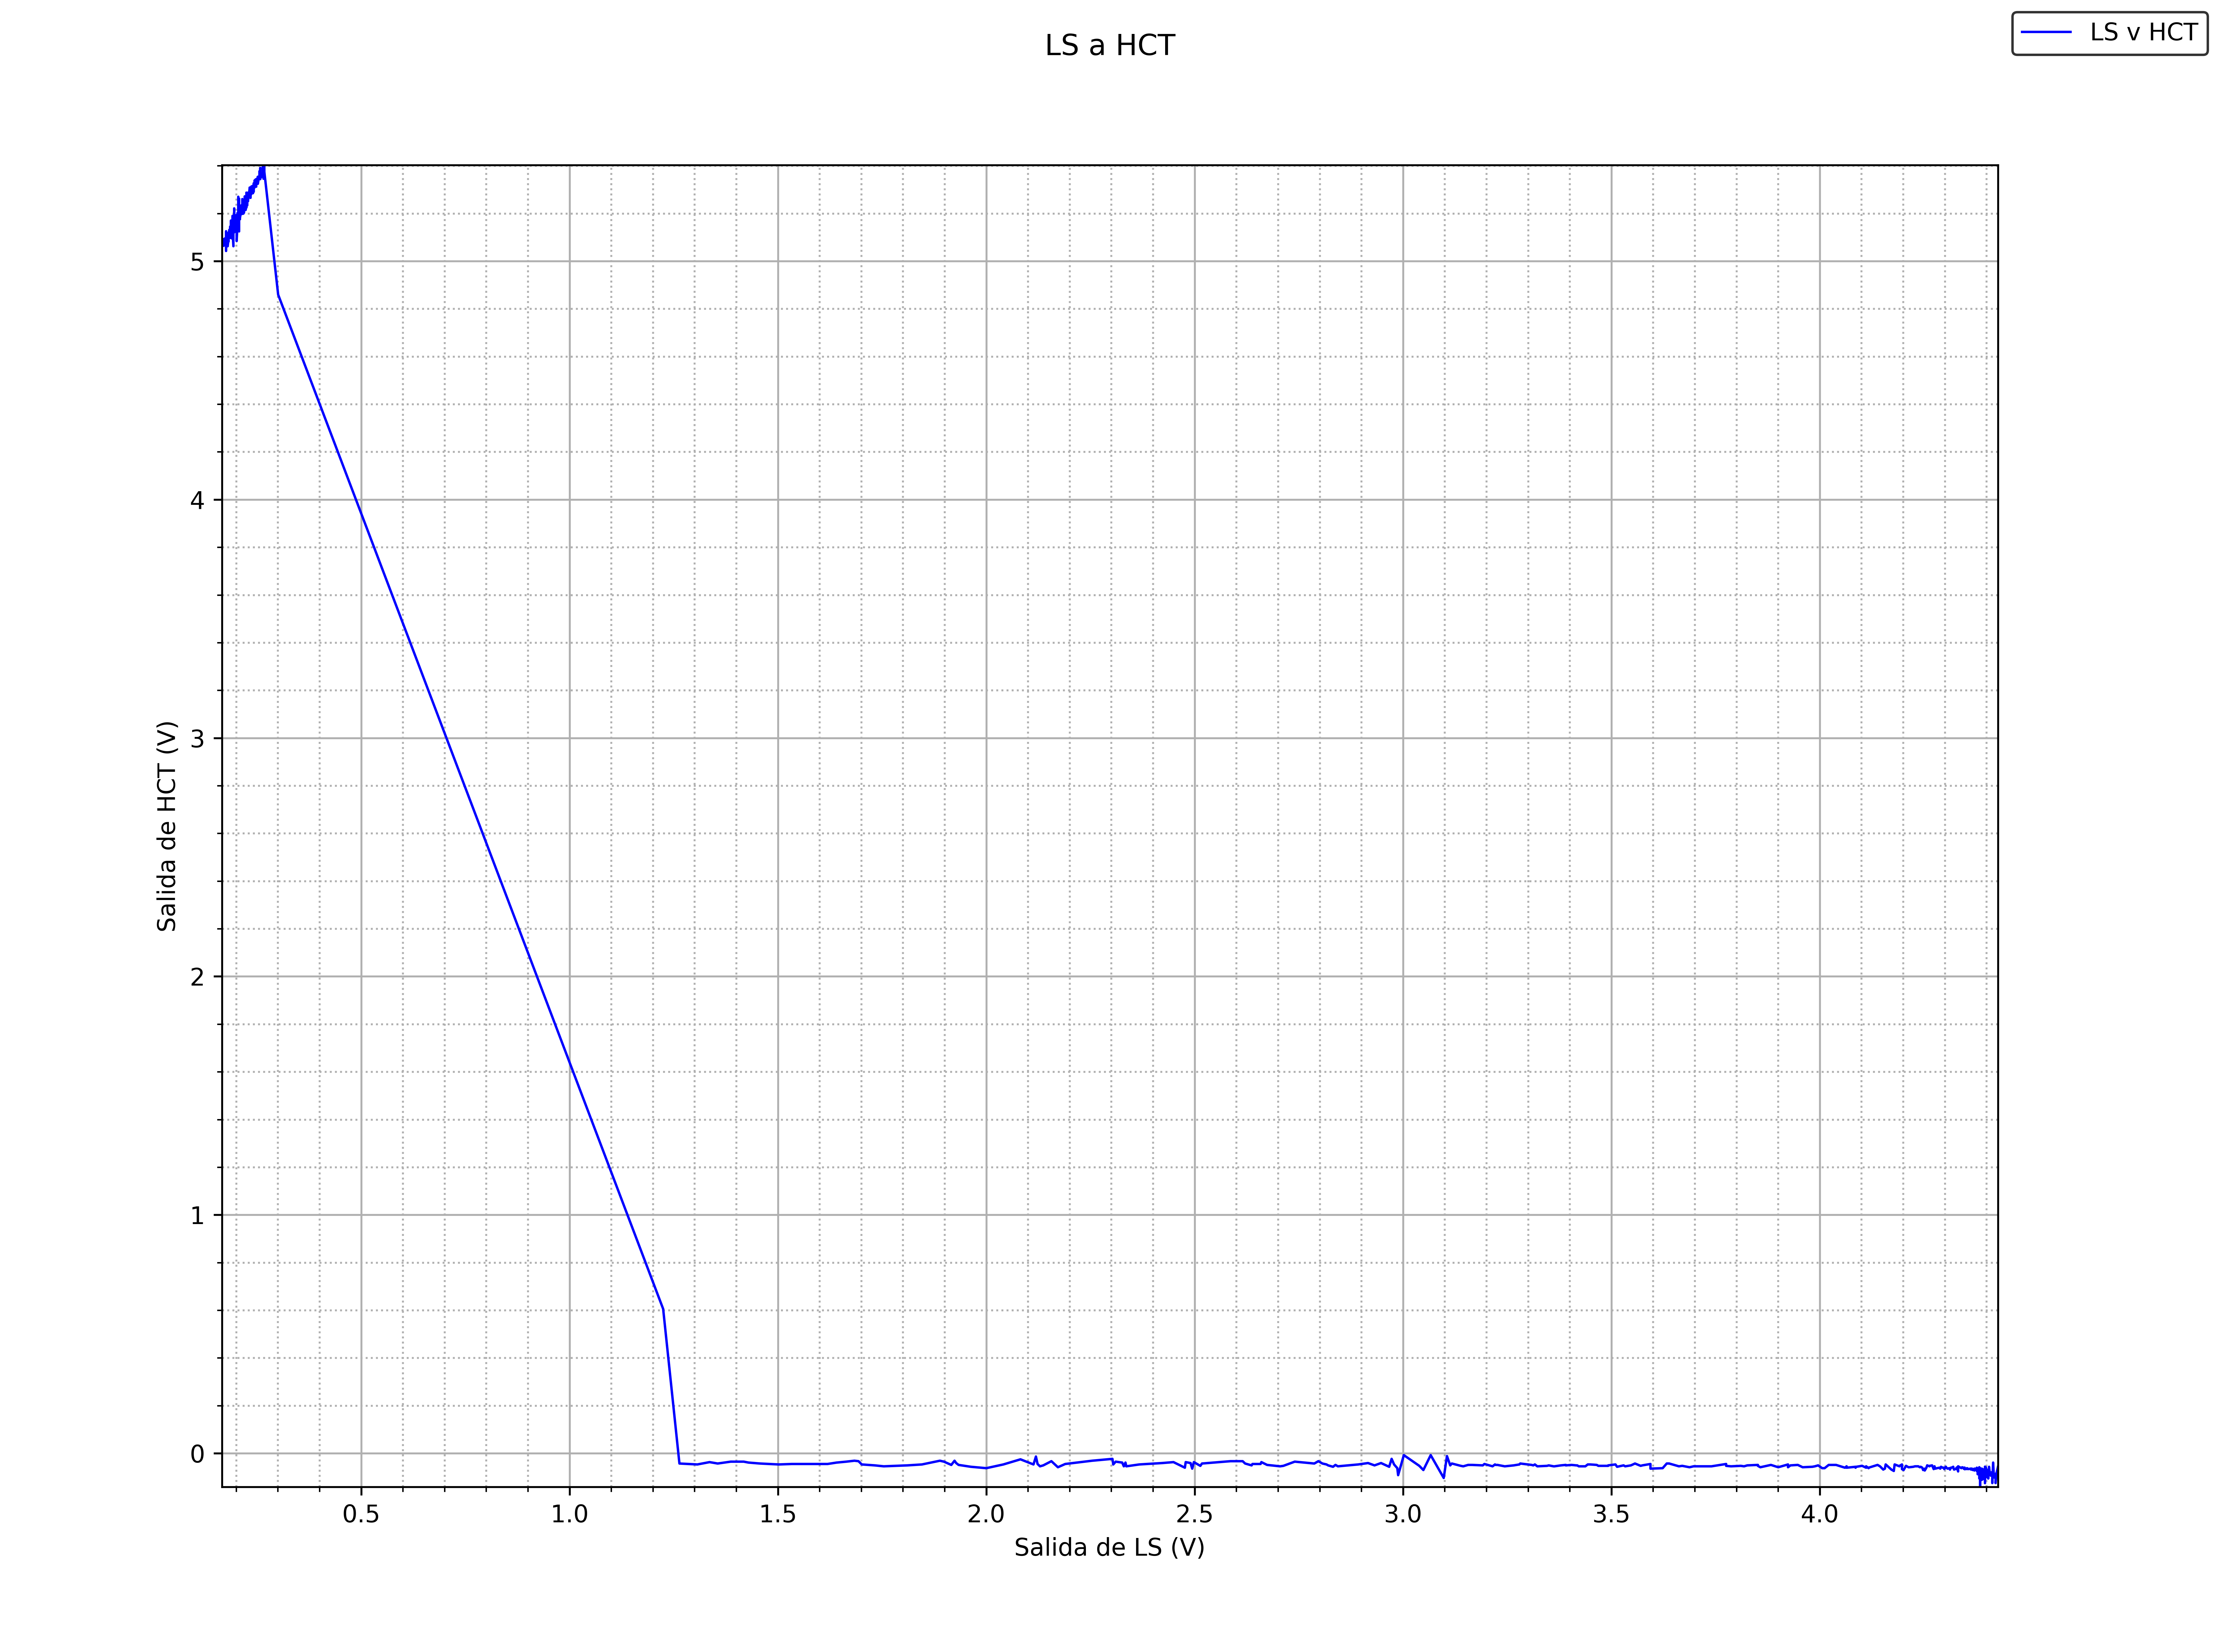
\includegraphics[width=0.5\textwidth]{../EJ2/Recursos/LS_H_v_HCT_L}
    \end{tabular}
    \caption{LS a HCT, con LS pasando de 1 a 0, y HCT de 0 a 1.}
    \label{fig:LS_H_v_HCT_L_ex5}
\end{figure}

Efectivamente lo esperado es lo que se obtiene en las mediciones, donde se puede apreciar una zona de indeterminación y oscilación en las transiciones de la configuración 
LS a HC.
Estos fenómenos no se observan luego en la configuración LS a HCT, en concordancia con lo estudiado de las hojas de datos, donde se aseguraba su compatibilidad.



\subsection{Conclusión}
A modo de cierre, se llega a la conclusión que la compatibilidad de tecnologías es un factor a tener en cuenta a la hora de realizar un diseño con compuertas lógicas de 
más de un tipo, si se quieren evitar estados indeterminados o glitches producto de transiciones con oscilaciones, causadas por incompatibilidades.
Se debe prestar especial atención al paso de tecnologías TTL a CMOS, y de ser necesario implementarlo, debe hacerse uso de compuertas CMOS especialmente diseñadas para 
esa aplicación, como lo son las de tipo HCT.

	\newpage
	\section{Ejercicio 3: Medici\'on de un glitch}

El prop\'osito de este apartado es analizar el comportamiento de un circuito l\'ogico determinado, implementado con compuertas f\'isicas. Dicho circuito corresponde a la tabla de verdad que se reproduce a continuaci\'on.

\begin{table}[H]
\centering
\label{tab:ej3_tabla_verdad}
\begin{tabular}{ccc|c}
A & B & C & Y \\ \hline
0 & 0 & 0 & 0 \\
0 & 0 & 1 & 1 \\
0 & 1 & 0 & 1 \\
0 & 1 & 1 & 1 \\
1 & 0 & 0 & 0 \\
1 & 0 & 1 & 1 \\
1 & 1 & 0 & 0 \\
1 & 1 & 1 & 0
\end{tabular}
\caption{Tabla de verdad}
\end{table}

\subsection{S\'intesis del circuito}
Para lograr el equivalente circuital de la tabla anterior se emplea un mapa de Karnaugh, de forma tal de lograr la expresi\'on m\'as simplificada, y por ende la de menor costo.

\begin{center}
    \begin{Karnaughvuit}
        \label{Karnaugh_glitch}
        \contingut{0,1,2,3,4,5,6,7}
        \implicant{3}{2}{green}
        \implicant{1}{5}{green}
	\end{Karnaughvuit}\\
Mapa de Karnaugh
\end{center}


Agrupando en mint\'erminos a los grupos resaltados en el mapa se llega a la siguiente expresi\'on:

\begin{equation}
\label{ej3_glitheq}
 Y = \overline{A}\cdot B + C \cdot \overline{B}
\end{equation}

En teor\'ia, el circuito resultante de \ref{ej3_glitheq} deber\'ia responder exactamente a la tabla de verdad. Observando el mapa de Karnaugh se puede concluir que existe la posibilidad de que suceda un glitch en la transici\'on del estado $(A = 0, B = 0, C = 1)$ al estado $(A = 0, B = 1, C = 1)$ (gr\'aficamente esto puede ser apreciado en la adyacencia existente entre los dos grupos). Es decir, es posible que la salida del circuito se comporte de forma inesperada, presentando por un instante un cero l\'ogico. Esta situaci\'on puede ser riesgosa si se tratara de un circuito l\'ogico real operando en su entorno de trabajo, dado que se podr\'ian desencadenar acciones indeseadas por parte de la etapa cuya entrada es el circuito que se analiza.

Para prevenir esto, se puede agregar un grupo extra que contenga las posiciones cuya transici\'on pudiera ser conflictiva. Si se implementa lo anterior se obtiene el siguiente mapa de karnaugh, con su correspondiente expresi\'on l\'ogica asociada.

\begin{center}

    \begin{Karnaughvuit}
        \label{Karnaugh_noglitch}
        \contingut{0,1,2,3,4,5,6,7}
        \implicant{3}{2}{green}
        \implicant{1}{5}{green}
        \implicant{1}{3}{blue}
\end{Karnaughvuit}\\
Mapa de Karnaugh correcci\'on de glitch
\end{center}

Los grupos que componen la soluci\'on de menor costo est\'an simbolizados en color verde, mientras que el grupo auxiliar est\'a marcado en azul.

\begin{equation}
\label{ej3_noglitheq}
 Y = \overline{A}\cdot B + C \cdot \overline{B} + \overline{A} \cdot C
\end{equation}

De esta forma, se asegura que la transici\'on entre las posiciones en conflicto sea la esperada, corrigiendo el problema. Como se puede observar, la ecuaci\'on~\ref{ej3_noglitheq} es la expresi\'on~\ref{ej3_glitheq} sumando al t\'ermino $\overline{A} \cdot C$. Se obtiene el circuito l\'ogico que se reproduce a continuaci\'on, resaltando en color verde las compuertas agregadas para implementar la correcci\'on.

\begin{figure}[H]
    \centering
    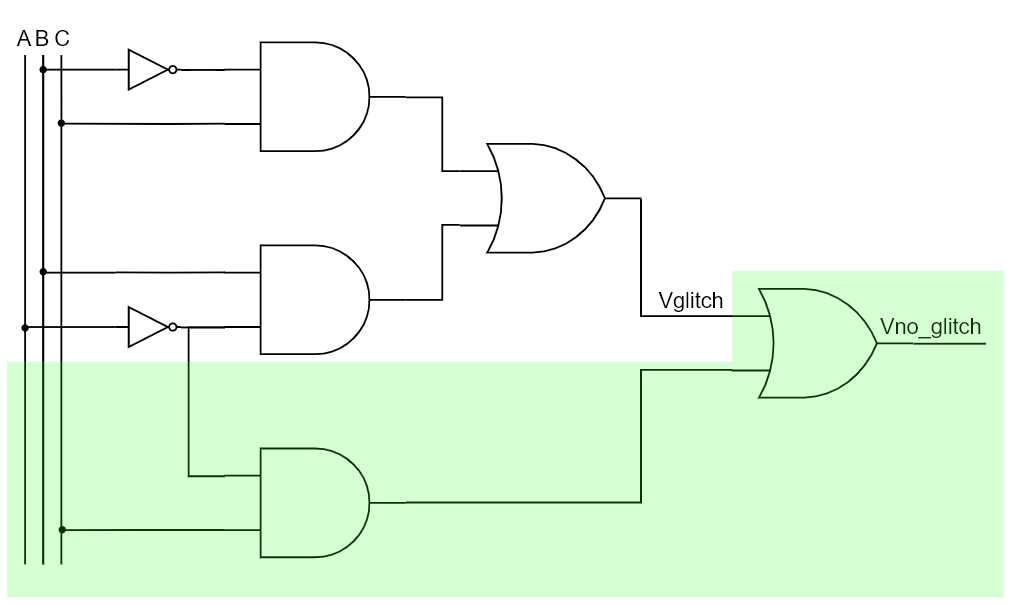
\includegraphics[width=0.9\textwidth]{../EJ3/Recursos/EJ3_logic_circuit.png}
	\caption{Circuito l\'ogico}
   	\label{fig:EJ3_logic_circuit}
\end{figure}

\subsection{Implementaci\'on y medici\'on del circuito}

Se arm\'o el circuito de la figura~\ref{fig:EJ3_logic_circuit} utilizando los siguientes integrados para cada tipo de compuerta l\'ogica.

\begin{table}[H]
    \centering
    \begin{tabular}{c c}
        Compuerta & Circuito integrado\\
        \hline
        $AND$ & $74HC08$ \\
        $OR$ & $74HC32$\\
        $NOT$ & $74HC04$\\
        \hline
    \end{tabular}
    \caption{IC empleados en implementaci\'on}
\end{table}

Se establecieron las condiciones de las entradas de tal forma de solo variar la variable \textsc{"B"}, emulando el cambio con una se\~nal cuadrada que oscila entre $0V$ y $5V$ a una frecuencia de $30kHz$. En primera instancia se observ\'o detalladamente el comportamiento de ambas salidas del circuito (con mint\'ermino de correcci\'on y sin el mismo) cuando el flanco de la se\~nal de entrada es ascendente. Se observan las siguientes respuestas (siendo la se\~nal de entrada color violeta, la se\~nal sin correcci\'on amarilla y la se\~nal con correcci\'on verde).

\begin{figure}[H]
    \centering
    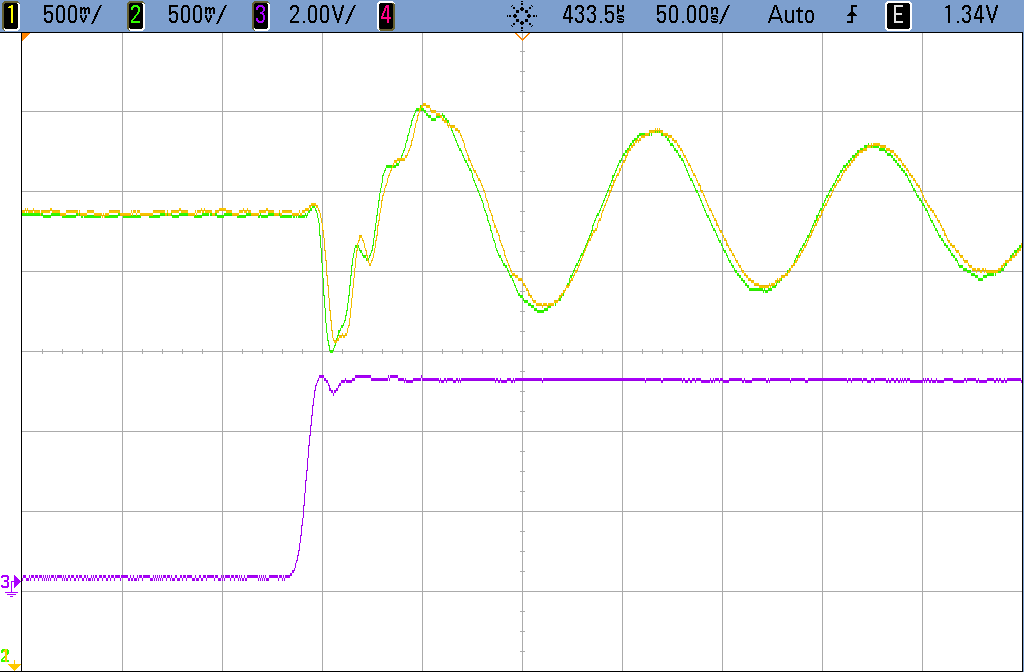
\includegraphics[width=0.9\textwidth]{../EJ3/Recursos/cropped_EJ3_positive_slope_response.png}
	\caption{Respuesta del circuito en flanco ascendente}
   	\label{fig:EJ3_positive_slope_response}
\end{figure}

En la figura anterior se puede apreciar una respuesta oscilatoria subamortiguada del circuito, destacando que ambas salidas presentan exactamente la misma oscilaci\'on. Se observa que en sus picos m\'aximos, las se\~nales de salida var\'ian entre $4V$ y $5.5V$. Estos niveles de tensi\'on se encuentran dentro del rango HIGH de una compuerta CMOS y de una del tipo TTL. De esta manera, no se puede considerar que exista un glitch en ninguna de las salidas.

An\'alogamente, se repiti\'o la medici\'on para un flanco descendente, reflejando los siguientes resultados (con la combinaci\'on de colores antes mencionada).

\begin{figure}[H]
    \centering
    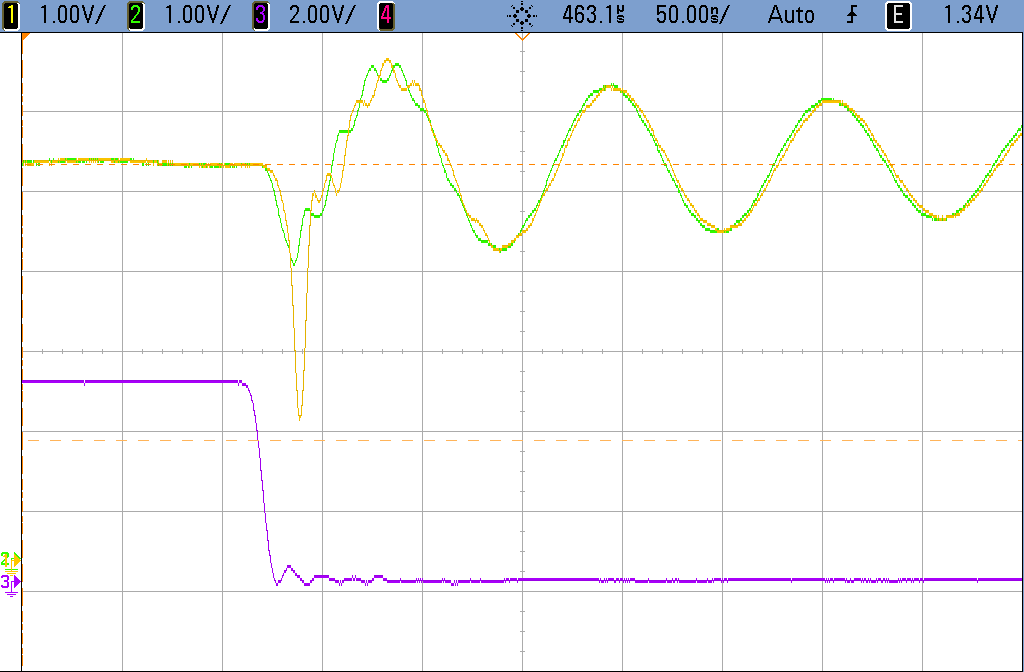
\includegraphics[width=0.9\textwidth]{../EJ3/Recursos/cropped_EJ3_negative_slope_response.png}
	\caption{Respuesta del circuito en flanco descendente}
   	\label{fig:EJ3_negative_slope_response}
\end{figure}

Para este caso s\'i se aprecia una diferencia razonable entre ambas respuestas: mientras que la oscilaci\'on de la salida compensada esta comprendida en un rango que va desde $3,8V$ hasta $5,8V$ (ambas dentro de los l\'imites aceptables de HIGH en ambas tecnolog\'ias), el l\'imite inferior del sobrepico de la salida sin compensar se acerca a $2,5V$. Este \'ultimo valor de tensi\'on se ubica por debajo de los rangos normales de entrada en HIGH, por lo que podr\'ia ser intepretada como un cero l\'ogico por el circuito cuya entrada es la salida de este. Asimismo, cabe destacar que el per\'iodo de duraci\'on del glitch es cercano a los $100 \mu s$, que es un tiempo relativamente corto. De todas formas, el impacto del glitch depender\'a de las caracter\'isticas del ciruito que reciba la se\~nal de salida de este. 

Este fen\'omeno se produce debido al tiempo de propagaci\'on de las entradas a trav\'es de las sucesivas etapas compuestas por compuertas l\'ogicas. Especialmente debido a que el camino circuital que recorren las se\~nales no les insume el mismo tiempo,  dado que es probable que una se\~nal determinada deba propagarse por m\'as compuertas que otras, gener\'andose una condici\'on de asimetr\'ia en el procesamiento. 

Por \'ultimo, se advierte que el tiempo en el que se estabiliza la oscilaci\'on es cercano a los $2,35ns$ como se aprecia en imagen de abajo.

\begin{figure}[H]
    \centering
    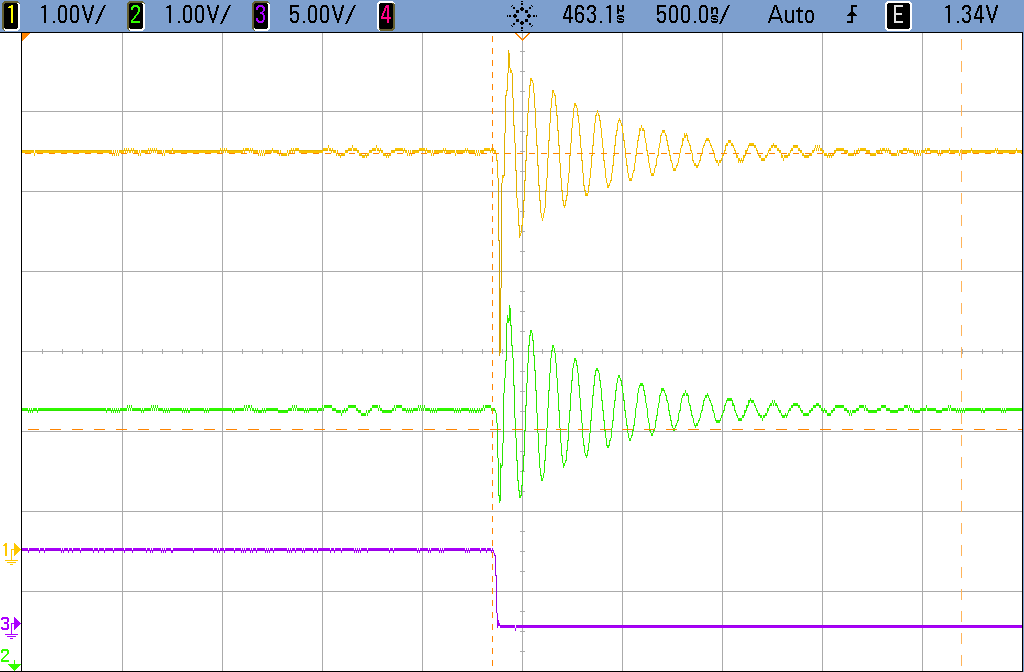
\includegraphics[width=0.9\textwidth]{../EJ3/Recursos/cropped_EJ3_negative_slope_response_zout.png}
	\caption{Respuesta del circuito en flanco descendente - Establecimiento}
   	\label{fig:EJ3_negative_slope_response_zout}
\end{figure}

\subsection{Conclusi\'on}
Como conclusi\'on, se puede destacar que el circuito sin compensar no ser\'ia seguro de implementar en una aplicaci\'on que requiera una alta confiabilidad del circuito. Dependiendo de la aplicaci\'on y del nivel de confiabilidad deseado se debe tener en cuenta el agregado del mint\'ermino de compensaci\'on, como se pudo observar con anterioridad.






	\newpage
	\section{Ejercicio 4: Tiempos de propagaci\'on en compuerta CMOS}
	\newpage
	\section{Ejercicio 5: TTL y MOS, entradas abiertas y compatibilidad entre tecnolog\'ias}

\subsection{Compuertas discretas con entrada desconectada}

\subsubsection{Descripci\'on general}
En la Fig. \ref{fig:open_gate_circuits} se muestra el esquema general bajo an\'alisis, se utiliza una compuerta AND de tecnolog\'ia TTL,
particularmente 74LS08 y una compuerta OR de tecnolog\'ia CMOS particularmente 74HC32. El objetivo es estudiar y comparar el comportamiento
cuando se deja una de las entradas sin un estado definido, obteniendo conclusiones sobre ello.

En el proceso de medici\'on se buscar\'a observar la entrada y salida de cada circuito, con la entrada al aire, o un estado bajo o alto y analizando
la susceptibilidad del mismo a fuentes de ruido externas o de interferencia. Se parte de la hip\'otesis de que el estado sin definir hace al circuito vulnerable
frente al ruido, y existen argumentos f\'isicos para sospechar que habr\'a mayor influencia en uno de los casos.

\begin{figure}[H]
    \centering
    \begin{tabular}{c c}
        \includegraphics[scale=0.8]{../EJ5/Recursos/ttl_open.png} &
        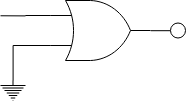
\includegraphics[scale=0.8]{../EJ5/Recursos/cmos_open.png}
    \end{tabular}
    \caption{Compuerta AND de tecnolog\'ia TTL y OR de tecnolog\'ia CMOS}
    \label{fig:open_gate_circuits}
\end{figure}

\subsubsection{Resultados}
En las Figs. \ref{fig:cmos_or_al_aire} y \ref{fig:ttl_and_al_aire} se observan los resultados de las mediciones, las cuales ordenadas de arriba hacia abajo y de izquierda a derecha, corresponden a la medici\'on
con entrada en estado bajo, en estado alto, con entrada al aire y luego con la mano apoyada. Para todos los casos la se\~nal amarilla corresponde a la entrada de la compuerta y la verde la salida.

Vale mencionar, que en los casos de estado bajo donde el valor promedio medido por el osciloscopio da negativo, se observ\'o con volt\'imetro digital que el valor era aproximadamente nulo y se atribuye
a defectos de la resoluci\'on digital del osciloscopio el asignar a tal magnitud un valor de dicho signo.

\begin{figure}[H]
    \centering
    \begin{tabular}{c c}
        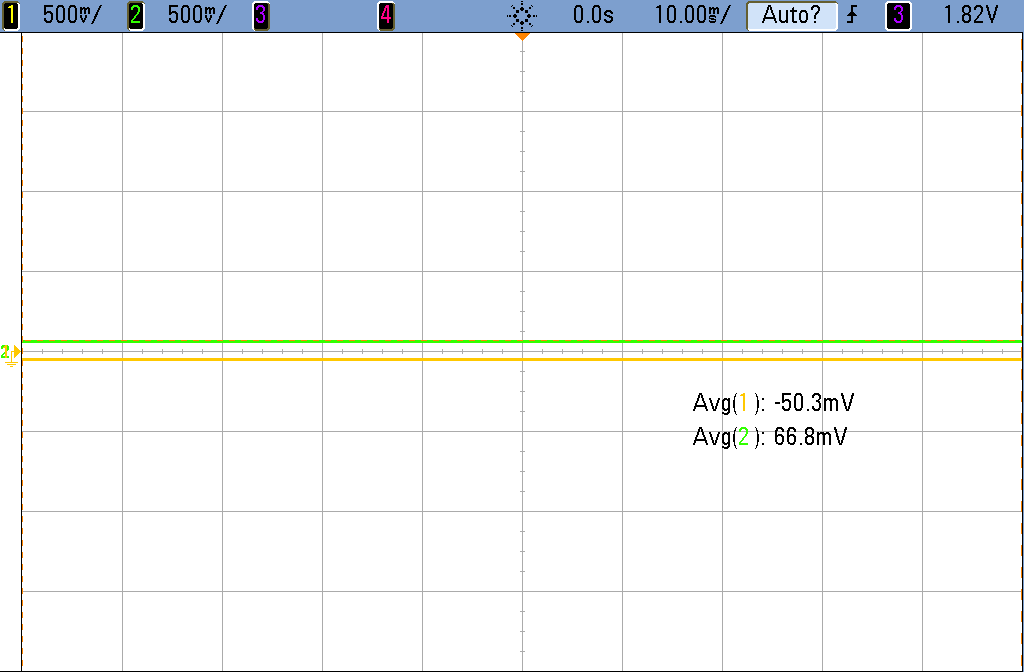
\includegraphics[scale=0.2]{../EJ5/Mediciones/Osciloscopio/CMOS_OR_SOLA/cropped_entrada_estado_bajo.png} &
        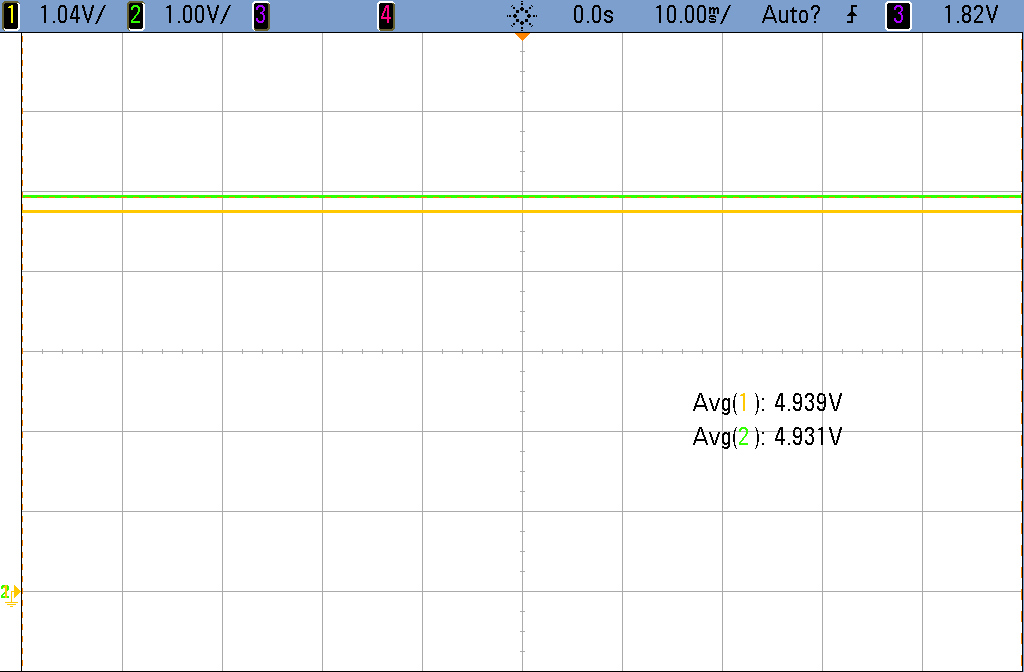
\includegraphics[scale=0.2]{../EJ5/Mediciones/Osciloscopio/CMOS_OR_SOLA/cropped_entrada_estado_alto.png} \\
        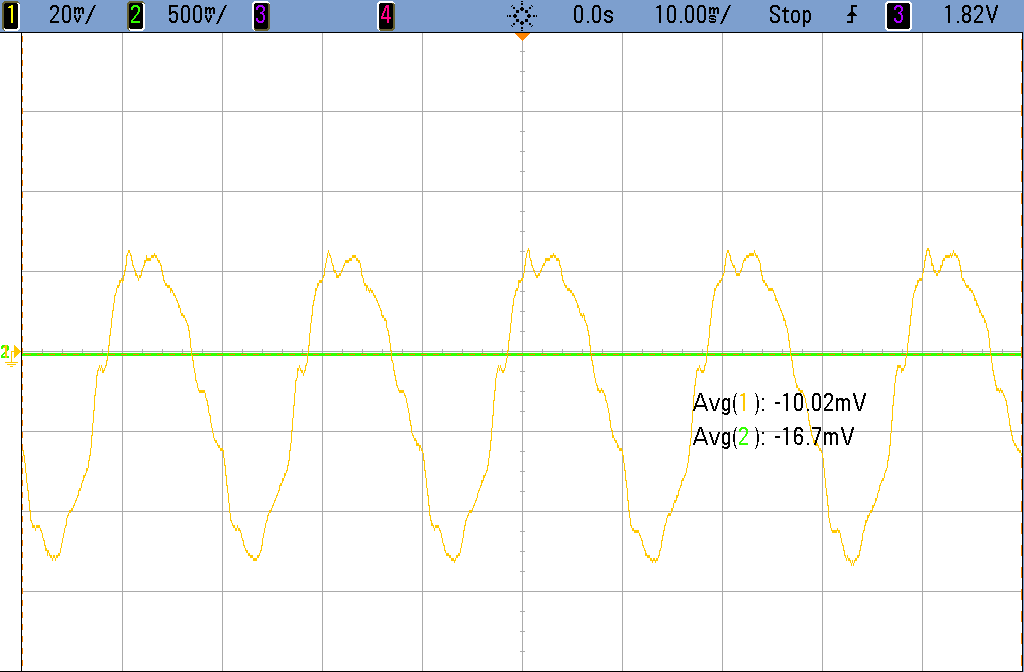
\includegraphics[scale=0.2]{../EJ5/Mediciones/Osciloscopio/CMOS_OR_SOLA/cropped_entrada_al_aire.png} &
        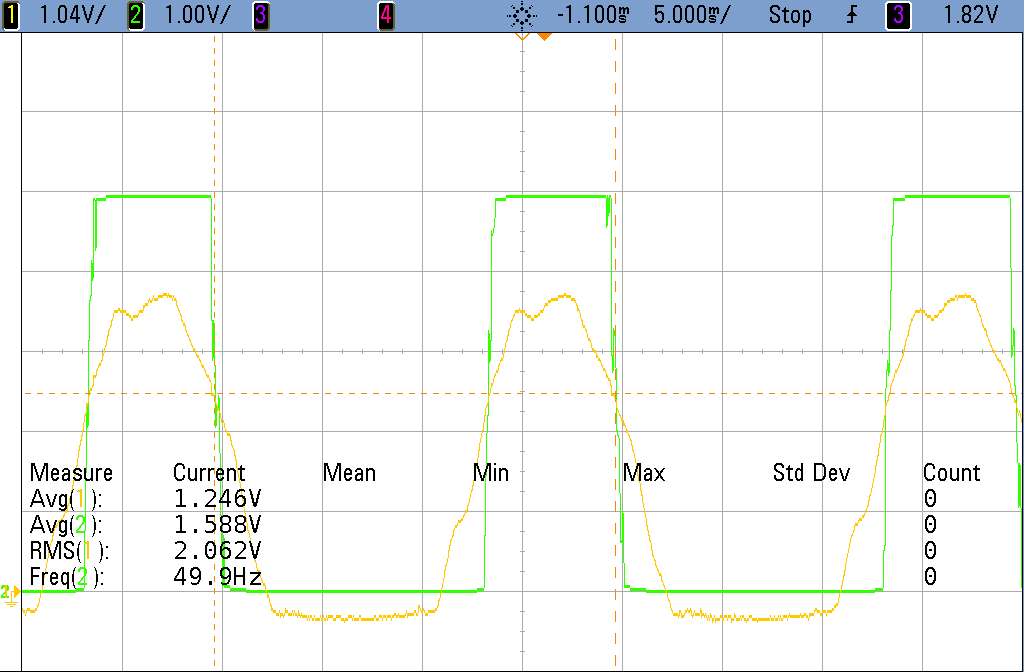
\includegraphics[scale=0.2]{../EJ5/Mediciones/Osciloscopio/CMOS_OR_SOLA/cropped_entrada_ruido.png} 
    \end{tabular}
    \caption{Mediciones para OR tecnolog\'ia CMOS modelo 74HC32}
    \label{fig:cmos_or_al_aire}
\end{figure}

\begin{figure}[H]
    \centering
        \begin{tabular}{c c}
            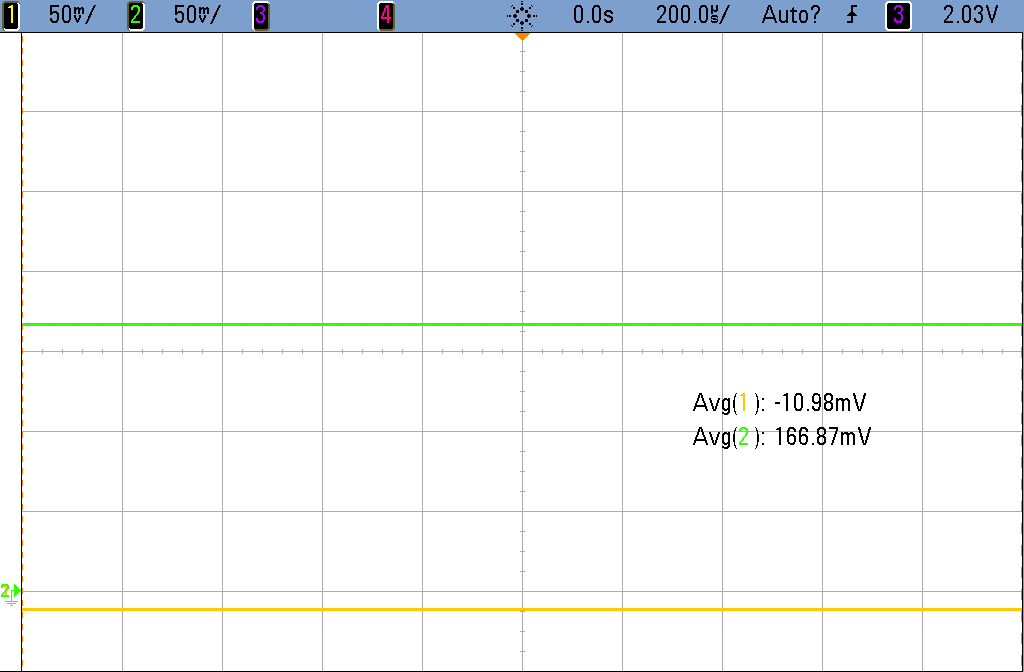
\includegraphics[scale=0.2]{../EJ5/Mediciones/Osciloscopio/TTL_AND_SOLA/cropped_entrada_estado_bajo.png} & 
            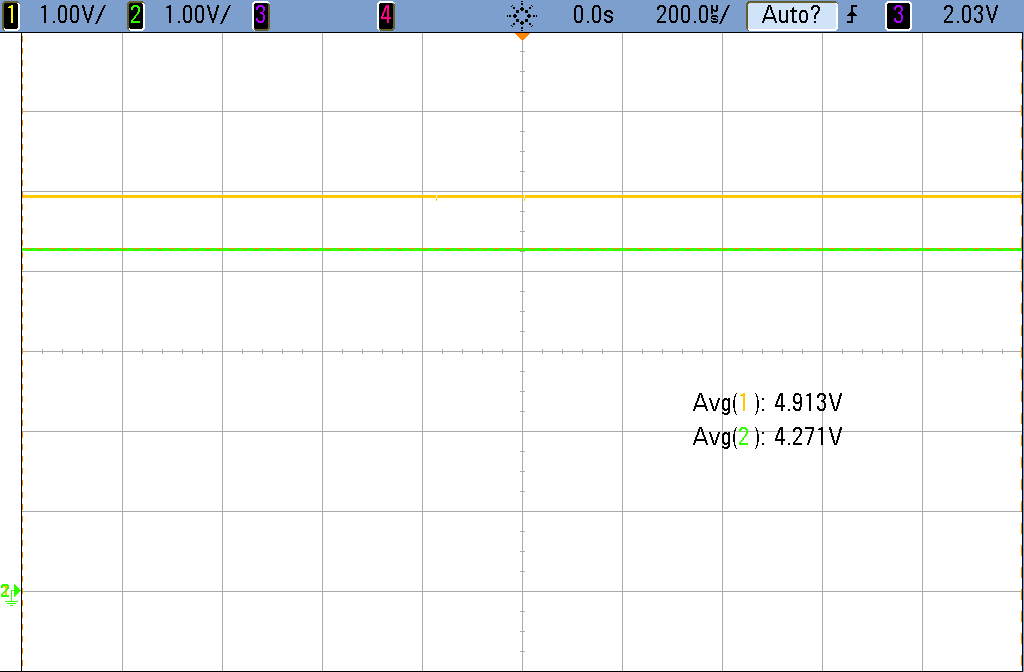
\includegraphics[scale=0.2]{../EJ5/Mediciones/Osciloscopio/TTL_AND_SOLA/cropped_entrada_estado_alto.png} \\ 
            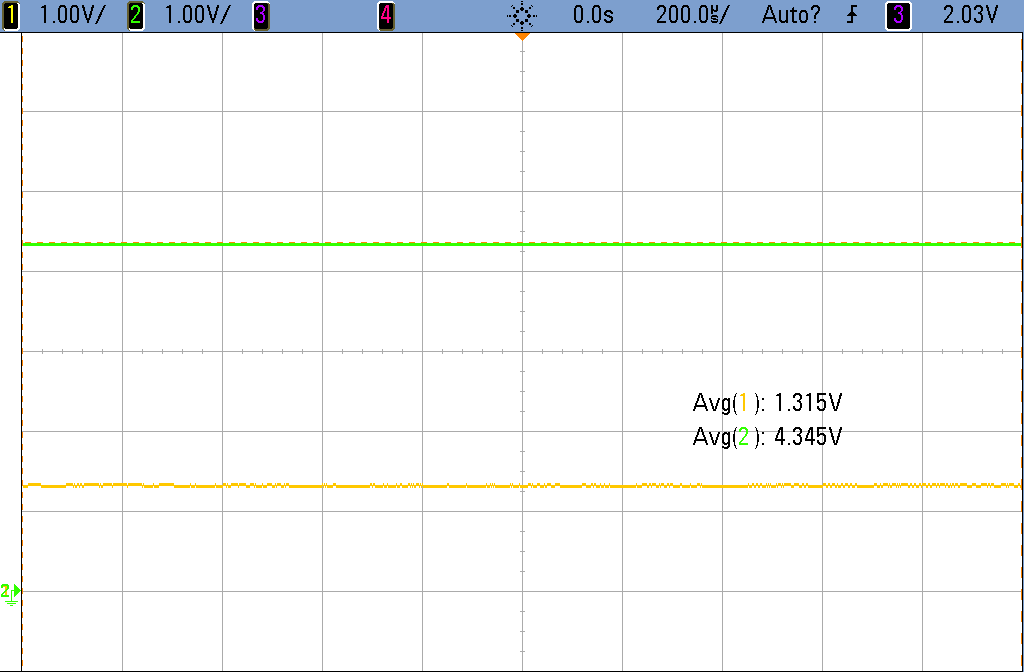
\includegraphics[scale=0.2]{../EJ5/Mediciones/Osciloscopio/TTL_AND_SOLA/cropped_entrada_al_aire.png} & 
            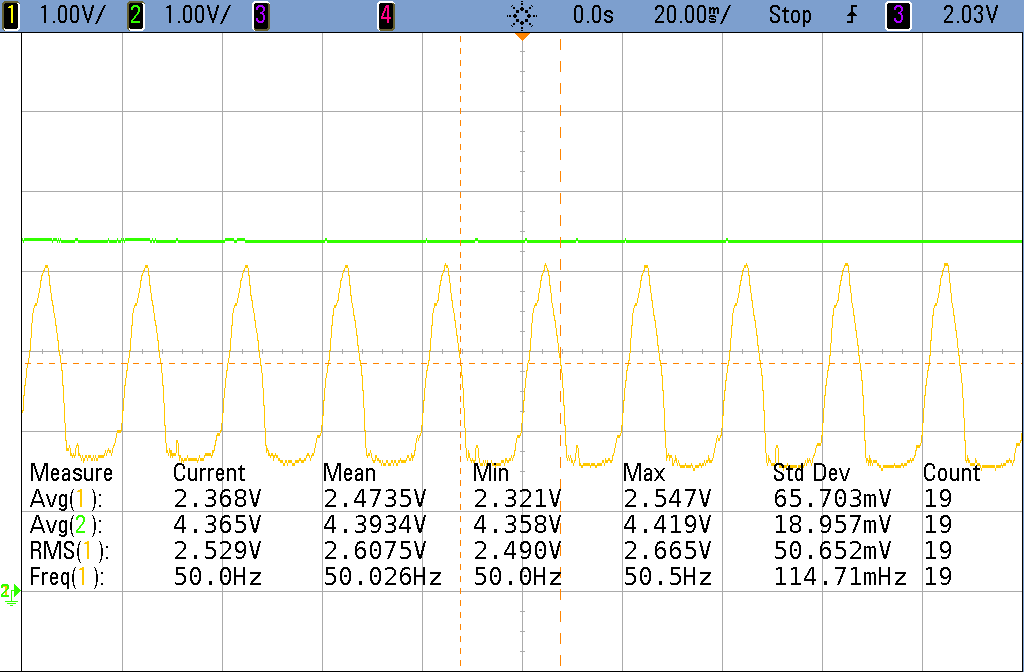
\includegraphics[scale=0.2]{../EJ5/Mediciones/Osciloscopio/TTL_AND_SOLA/cropped_entrada_ruido_frecuencia.png}  
        \end{tabular}
    \caption{Mediciones para AND tecnolog\'ia TTL modelo 74LS08}
    \label{fig:ttl_and_al_aire}
\end{figure}

\subsubsection{An\'alisis de resultados}
En primer lugar, se puede observar que para cada tecnolog\'ia los estados alto y bajo tienen diferente nivel de tensi\'on, lo cual
era esperado a partir de los datos provistos por el fabricante denominados como $V_{OH}$ y $V_{OL}$.

Luego, en principio cuando la entrada se encuentra al aire se puede observar una mayor inmunidad de la tecnolog\'ia TTL frente al ruido,
dado que su valor si bien es indefinido, se mantiene casi constante $V_{IN} \approx 1.315V$, y dado que $V_{IL} = 0.8V < 1.315V < 2V = V_{IH}$ esto indica que
tal nivel se encuentra en donde no est\'a asegurado el comportamiento de la compuerta y por ello la salida tiene tal resultado. Por otro lado, para la entrada al aire,
se puede observar que en la compuerta CMOS hay una oscilaci\'on de la entrada con valor acotados que no producen un cambio sobre la salida.
Esta diferencia entre tecnolog\'ias con una entrada al aire es consecuencia directa de las caracter\'isticas f\'isicas de los transistores MOS, en los cuales la aislaci\'on el\'ectrica
del Gate produce una impedancia de entrada muy elevada para la cual una fuente de ruido de corriente puede producir variaciones de tensi\'on apreciables. Esto \'ultimo puede verse de forma m\'as notoria
cuando se apoya la mano sobre los contactos, ante lo cual el ruido aumenta y la compuerta CMOS recibe una entrada significativa que produce cambios de estado que dan lugar a una oscilaci\'on de la salida,
mientras que en el caso de TTL la se\~nal de ruido no produce un cambio significativo sobre la salida.

Por \'ultimo, es importante aclarar que no es arbitrario que la frecuencia de oscilaci\'on sea aproximadamente $50Hz$, dado que es el ruido de la l\'inea el\'ectrica el que se ve introducido al circuito.

\begin{figure}[H]
    \centering
    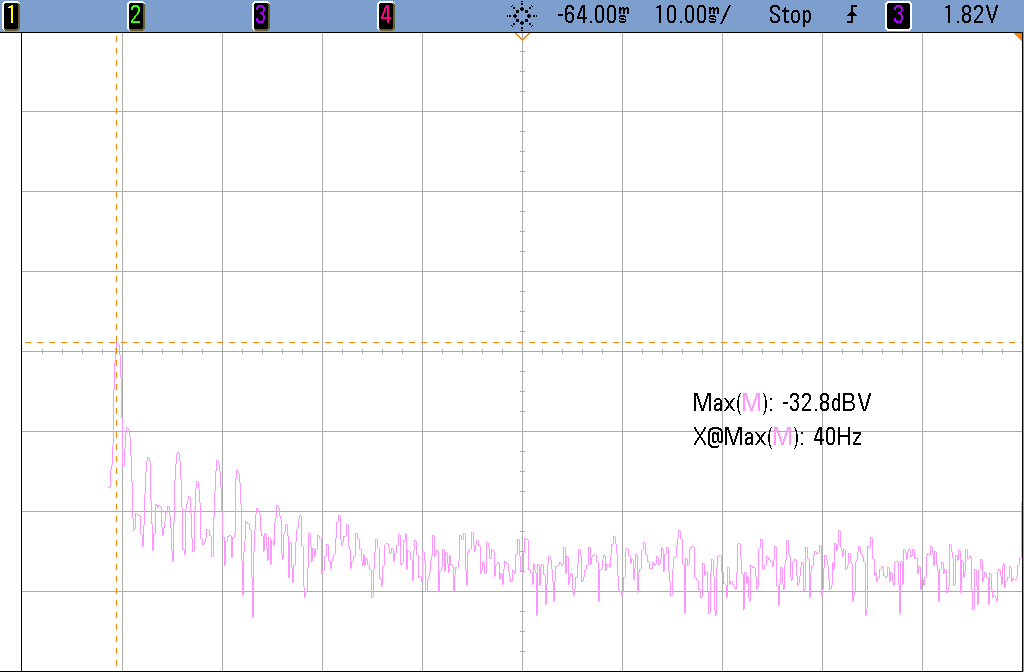
\includegraphics[scale=0.3]{../EJ5/Mediciones/Osciloscopio/CMOS_OR_SOLA/cropped_fft_ruido_contacto.png}
    \caption{FFT aplicada sobre la se\~nal de entrada con la mano apoyada}
    \label{fig:fft_mediciones}
\end{figure}

\subsection{Conexi\'on TTL y CMOS}

\subsubsection{Descripci\'on general}
En la Fig. \ref{fig:ttl_cmos_connected} se ilustra el esquema general del circuito a analizar en esta parte, en la cual el objetivo es analizar el comportamiento
del circuito resultante, partiendo de la base donde la salida ser\'a igual a la entrada aplicando axiomas del algebra booleana.

Se parte de la hip\'otesis de que este circuito podr\'ia presentar un comportamiento alejado del esperado, dado que las tensiones de la tecnolog\'ia TTL y CMOS no son completamente compatibles,
puesto que seg\'un los datos provistos por el fabricante, la TTL entrega una tensi\'on m\'inima de estado alto en $V_{OH} = 2.7V$ mientras que la entrada m\'inima detectada como un estado alto para
CMOS es $V_{IH} = 3.15V$. Para los escenarios del rango intermedio, el circuito se comportar\'a de manera indeterminada.

Se propone realizar mediciones con el objetivo de encontrar las condiciones l\'imite para las cuales se alcanza el problema mencionado anteriormente, puesto que se posible que particularmente la 
compuerta empleada caiga dentro del margen donde el funcionamiento es el esperado. Por esto \'ultimo es que se realizar\'an mediciones con valores de continua, con una se\~nal cuadrada de diversas frecuencias,
y cargando con resistencias o capacitores la salida de las compuertas. Estos procesos buscan simular las exigencias de un circuito sobre la compuerta, llev\'andola al l\'imite para observar que del rango garantizado
por el fabricante en el cual deber\'ia funcionar, el resultante menor.


Es importante aclarar que en la interconexi\'on de compuertas l\'ogicas discretas, es de inter\'es analizar si las corrientes de consumo no superan los valores m\'aximos para cada estado
de la compuerta empleada, no obstante no es un inconveniente en el caso de estudio ya que CMOS por su gran impedancia de entrada posee una corriente de p\'erdida muy inferior a la capacidad
m\'axima de la TTL.

\begin{figure}[H]
    \centering
        \includegraphics[scale=0.6]{../EJ5/Recursos/connection.png}
    \caption{Circuito l\'ogico a ensayar}
    \label{fig:ttl_cmos_connected}
\end{figure}

\subsubsection{Resultados}
En las Figs. \ref{fig:circuit_complete_measures} las se\~nales de color amarillo corresponden a las entradas, las verdes a la salida y luego las de color morado
fueron empleadas para ilustrar el estado de la se\~nal entre ambas compuertas. Las figuras est\'an ordenadas de arriba hacia abajo, de izquierda a derecha, en el orden
de la medici\'on para el estado bajo, estado alto, entrada al aire, con una carga resistiva baja, alta y excedida en la salida TTL.

\begin{figure}[H]
    \centering
    \begin{tabular}{c c}
        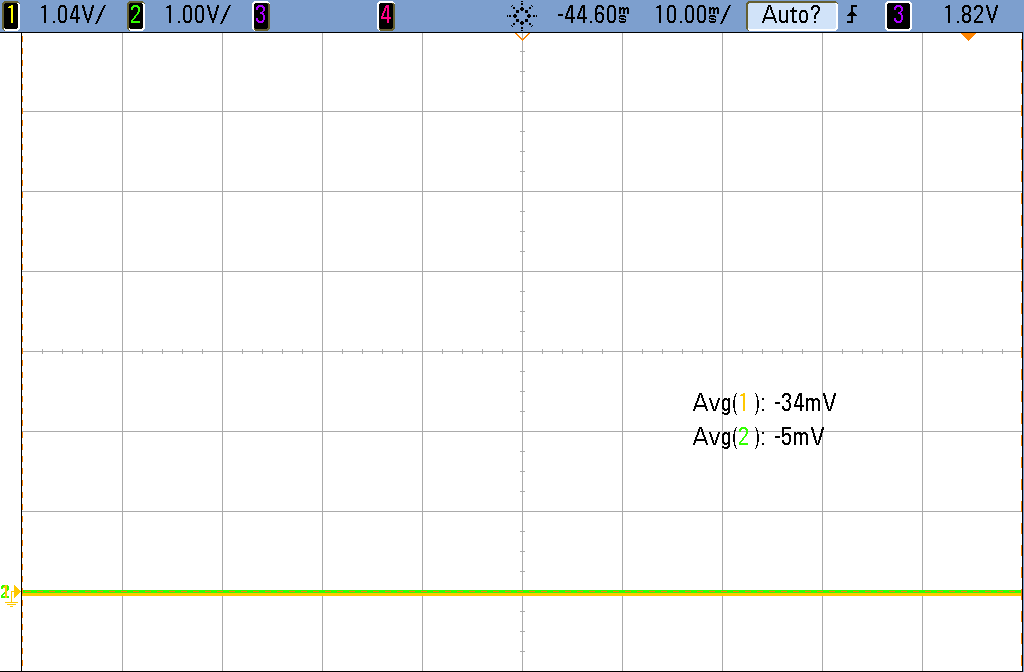
\includegraphics[scale=0.2]{../EJ5/Mediciones/Osciloscopio/CONEXION/cropped_entrada_estado_bajo.png} &
        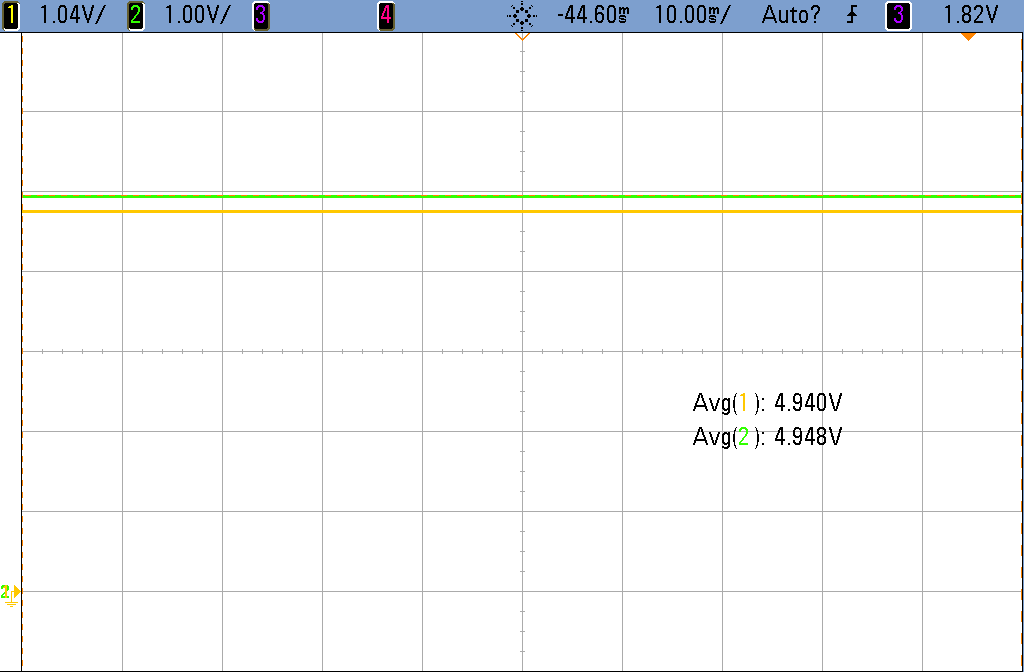
\includegraphics[scale=0.2]{../EJ5/Mediciones/Osciloscopio/CONEXION/cropped_entrada_estado_alto.png} \\
        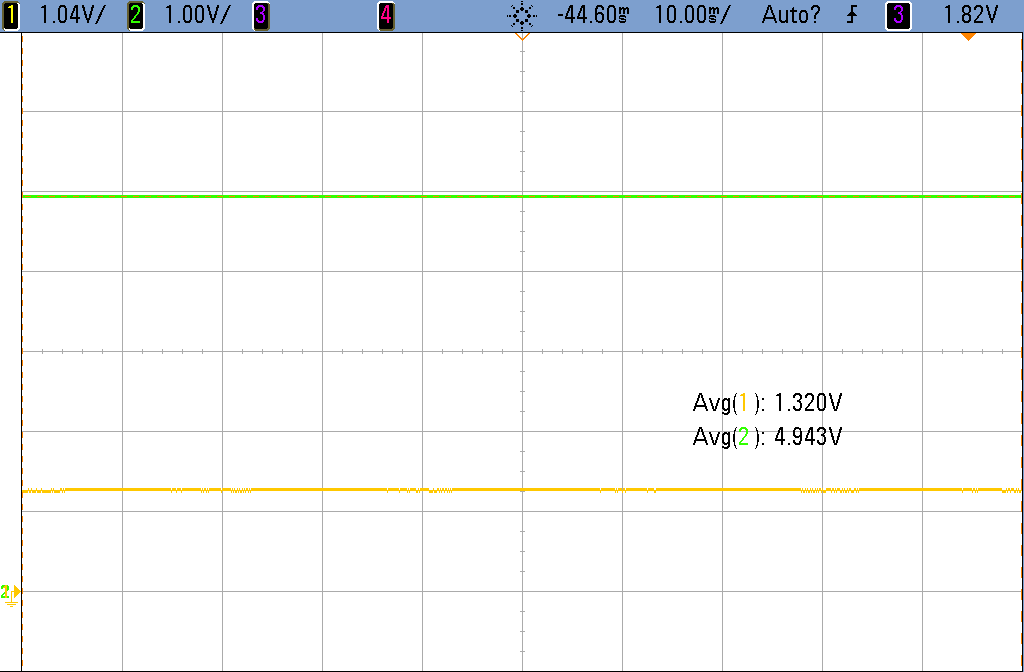
\includegraphics[scale=0.2]{../EJ5/Mediciones/Osciloscopio/CONEXION/cropped_entrada_al_aire.png} &
        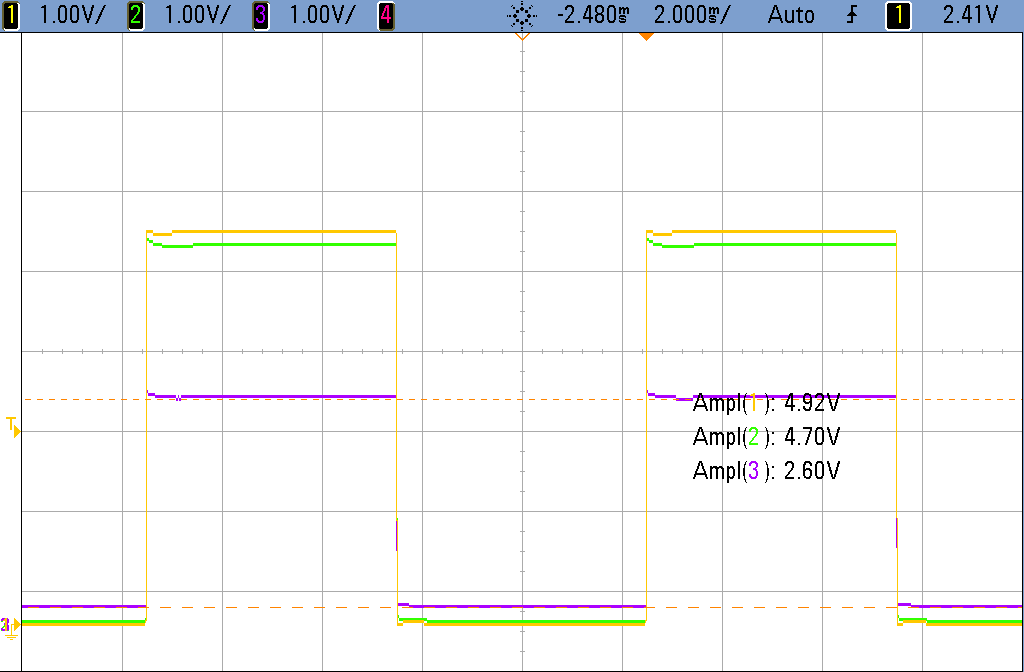
\includegraphics[scale=0.2]{../EJ5/Mediciones/Osciloscopio/CONEXION/cropped_con_carga_baja.png} \\
        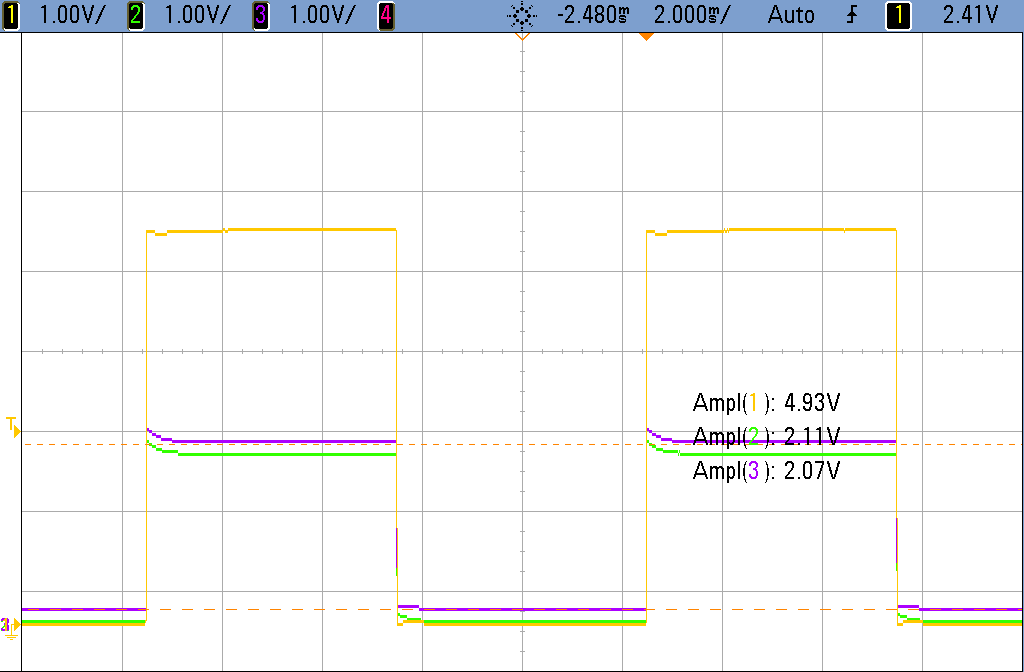
\includegraphics[scale=0.2]{../EJ5/Mediciones/Osciloscopio/CONEXION/cropped_con_carga_alta.png} &
        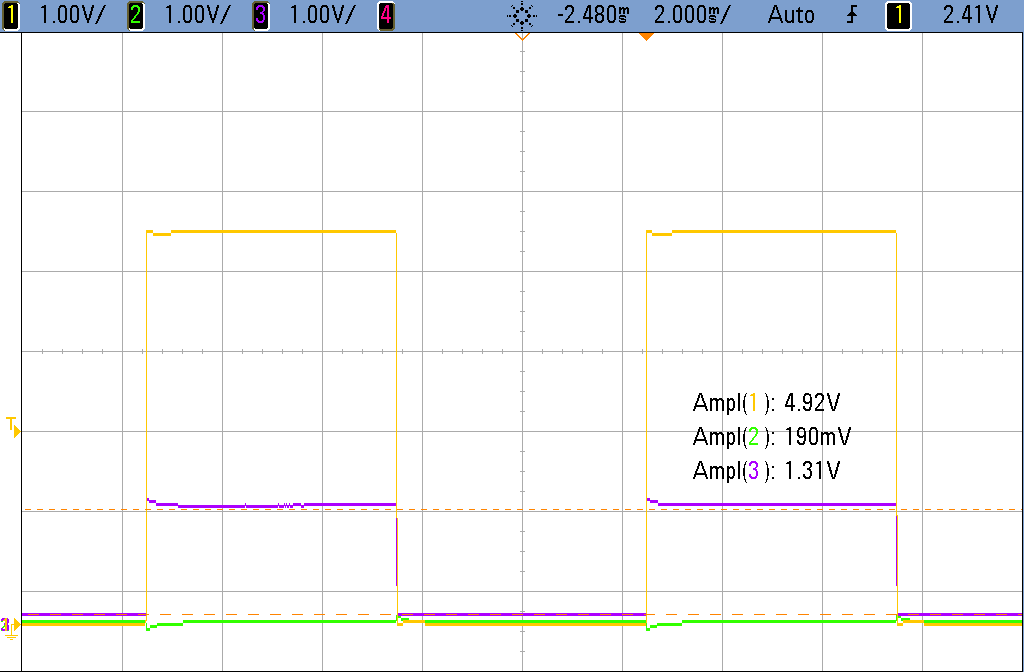
\includegraphics[scale=0.2]{../EJ5/Mediciones/Osciloscopio/CONEXION/cropped_con_carga_excedida.png} \\
    \end{tabular}
    \caption{Mediciones del circuito completo}
    \label{fig:circuit_complete_measures}
\end{figure}

\subsubsection{An\'alisis de resultados}
De los resultados obtenidos puede concluirse que en verdad bajo condiciones donde no se requiere mucho consumo de corriente, entre otras cosas,
la conexi\'on realizada entre una compuerta TTL y una compuerta CMOS es compatible, no obstante, al momento de simular exigencias de corriente por la conexi\'on
de m\'ultiples circuitos, luego los niveles de tensi\'on de la TTL comienzan a bajar cercanos a lo que el fabricante garantiza que sigue siendo un estado alto,
no obstante no es compatible con lo que CMOS reconoce como tal, por lo tanto deja de funcionar como se espera.

Se a\~naden algunas mediciones adicionales que se realizaron en la b\'usqueda de los l\'imites de funcionamiento. Entre estas, se analiz\'o qu\'e suced\'ia
con una se\~nal triangular para ver c\'omo respond\'ian los niveles de tensi\'on de cada tecnolog\'ia, y para altas frecuencias c\'omo afectaban las cargas capacitivas
y los tiempos de propagaci\'on de entrada a salida.

\begin{figure}[H]
    \centering
        \begin{tabular}{c c}
            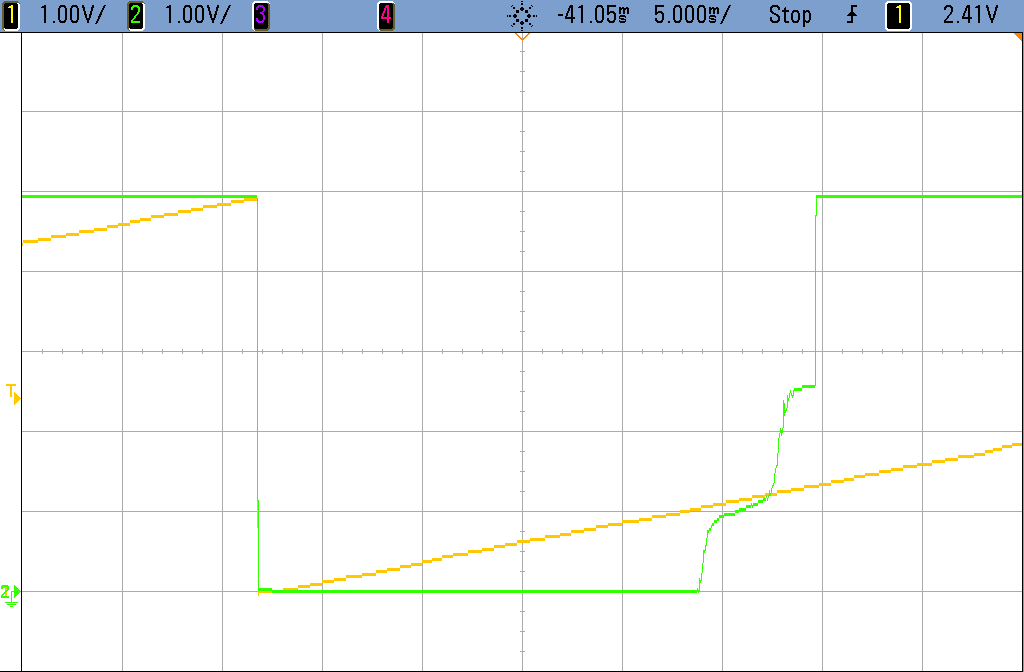
\includegraphics[scale=0.2]{../EJ5/Mediciones/Osciloscopio/CONEXION/cropped_triangular_zoom.png} &
            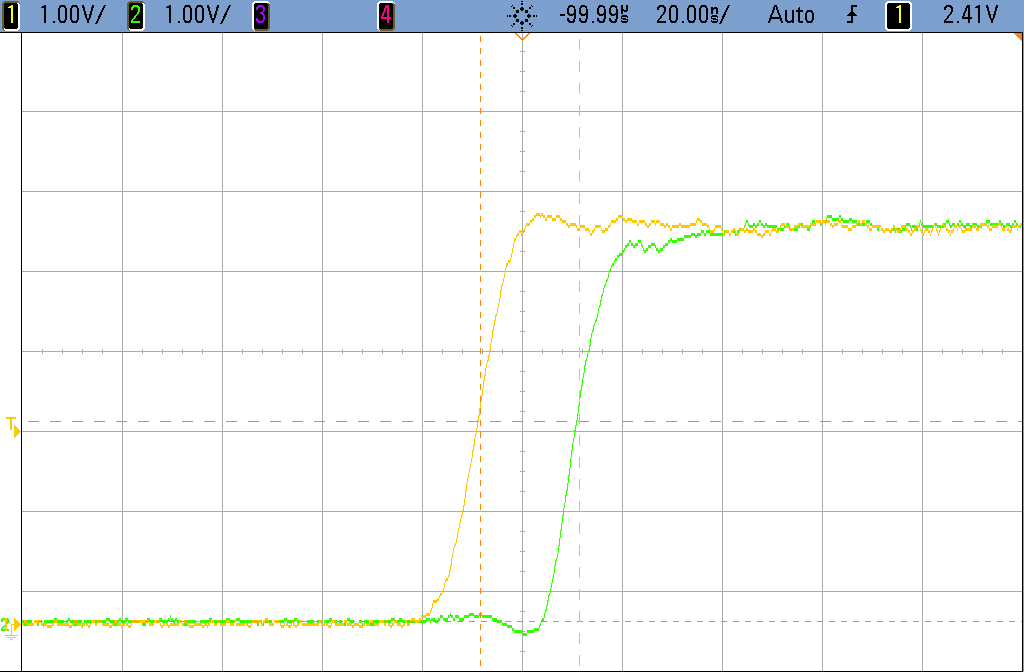
\includegraphics[scale=0.2]{../EJ5/Mediciones/Osciloscopio/CONEXION/cropped_propagacion.png} \\
        \end{tabular}
        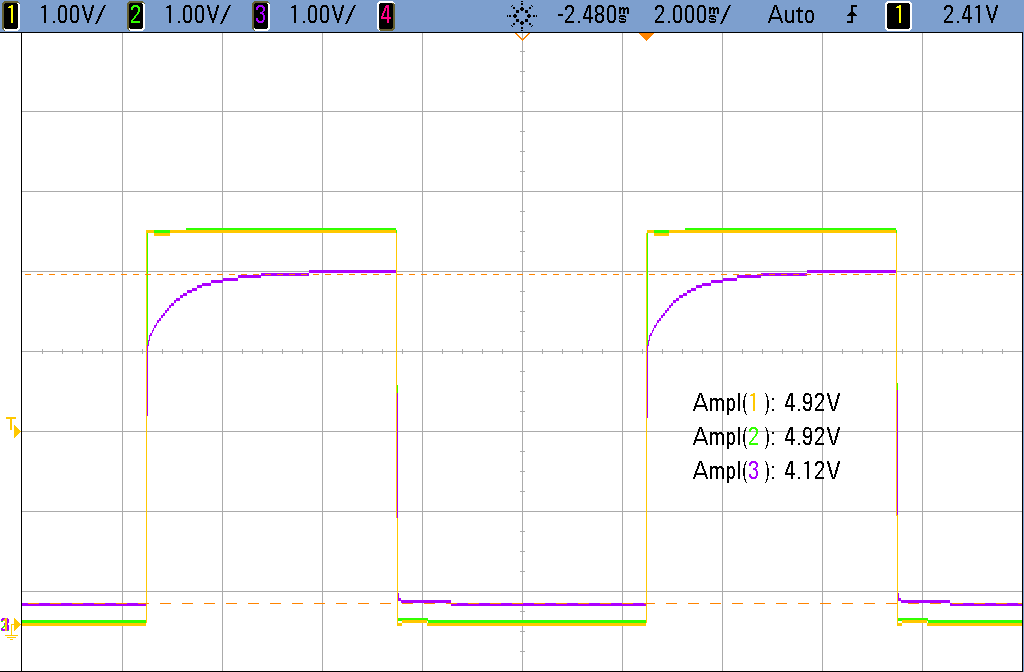
\includegraphics[scale=0.2]{../EJ5/Mediciones/Osciloscopio/CONEXION/cropped_carga_capacitiva.png}
    \caption{Mediciones adicionales}
    \label{fig:additional_measures}
\end{figure}

\subsubsection{Soluciones propuestas}
En las Figs. \ref{fig:circuitos_soluciones} se pueden observar dos circuitos diferentes propuestos como soluci\'on al problema del nivel de tensi\'on para los estados l\'ogicos de una TTL con una CMOS.
Se comparan ambas soluciones dado que la segunda de ellas implementada con un MOSFET es bidireccional, con lo cual la interfaz permite el cambio de nivel en ambos sentidos, pero adem\'as por el hecho de que
permite definir un cambio de nivel de diferentes tensiones. Por el otro lado, la implementaci\'on del circuito con un BJT tipo PNP \'unicamente permite hacer una adaptaci\'on para corregir el nivel de tensi\'on sin cambiarlo,
ya que de otra forma no funcionar\'ia, por ejemplo si se buscara pasar de $3.3V$ a $5V$.

\begin{figure}[H]
    \centering
    \begin{tabular}{c c}
        \includegraphics[scale=0.4]{../EJ5/Recursos/pnp_interface.png} &
        \includegraphics[scale=0.4]{../EJ5/Recursos/mos_interface.png}
    \end{tabular}
    \caption{Circuitos propuestos}
    \label{fig:circuitos_soluciones}
\end{figure}

En las Figs. \ref{fig:resultados_interfaces} la se\~nal amarilla corresponde a la entrada de los circuitos de interfaz, mientras que la morada
corresponde a la salida de los mismos. En la izquierda se observa el resultado de la interface PNP y en la derecha la de NMOS, se puede deducir claramente
que la implementaci\'on de mejor rendimiento es la MOS ya que logra mejor niveles de tensi\'on para cada estado.

\begin{figure}[H]
    \centering
    \begin{tabular}{c c}
        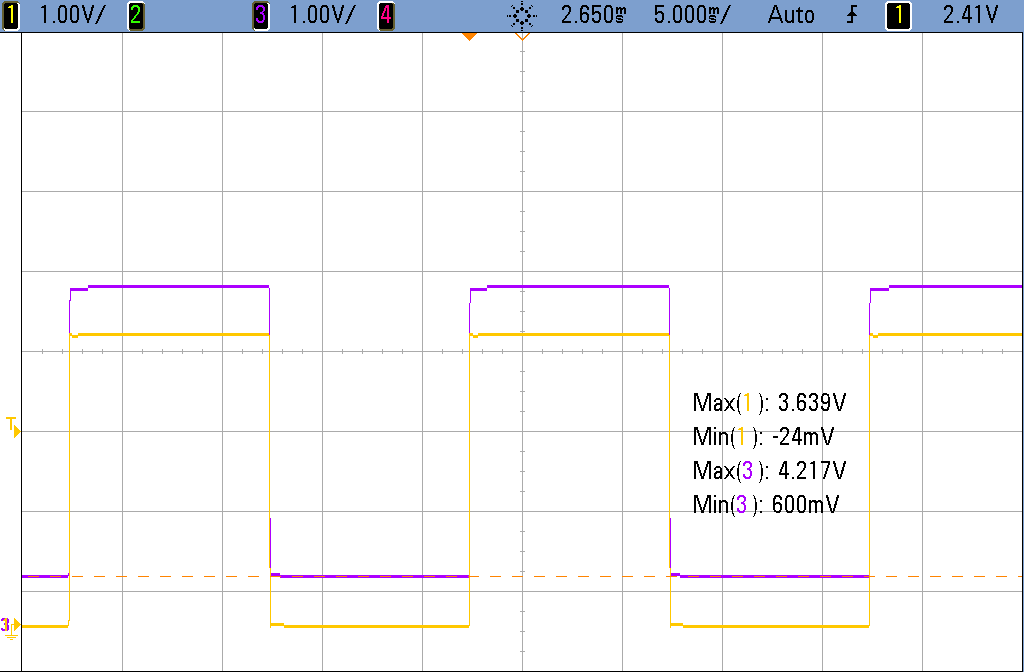
\includegraphics[scale=0.2]{../EJ5/Mediciones/Osciloscopio/LEVEL_SHIFTER/cropped_bjt.png} &
        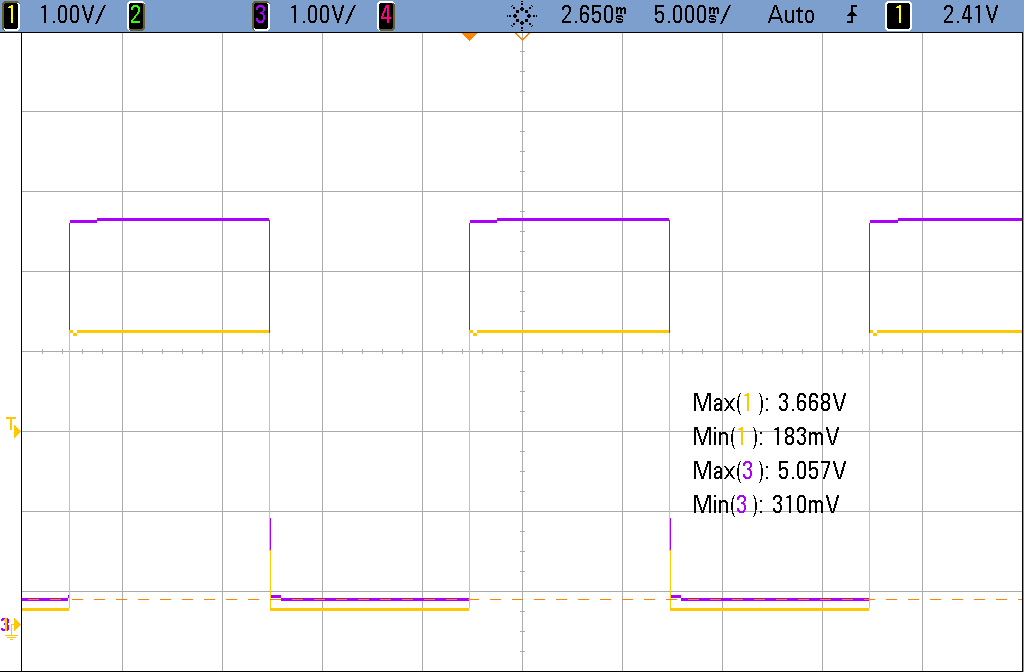
\includegraphics[scale=0.2]{../EJ5/Mediciones/Osciloscopio/LEVEL_SHIFTER/cropped_mos.png} 
    \end{tabular}
    \caption{Resultados de los circuitos implementados ante una se\~nal cuadrada con valores arbitrarios}
    \label{fig:resultados_interfaces}
\end{figure}

\subsection{Conclusi\'on}
Las tecnolog\'ias TTL y CMOS, como se ha visto, difieren en numerosos aspectos que se utilizan para caracterizar el comportamiento de una compuerta l\'ogica, no obstante, usualmente s\'olo se tienen en cuenta niveles de tensi\'on, corrientes m\'aximas de consumo e incluso tiempos de retardo en los procesos de transici\'on. A pesar de esto, la inmunidad al ruido o la susceptibilidad al mismo suele ser un aspecto a tener en cuenta, sobre todo en tecnolog\'ias MOS donde por su construcci\'on
f\'isica pueden darse los fen\'omenos antes vistos.



	\newpage
	\section{Dise\~no e implementaci\'on multivibradores}
	\newpage
	\section{Ejercicio 7: Dise\~no de contadores sincr\'onicos y asincr\'onicos de 3 bits}

\subsection{Contador Asincr\'onico}
En esta secci\'on se propone el dise\~no de un contador asincr\'onico de 3 bits ascendente empleando \'unicamente Flip Flops D, puesto que es el \'unico tipo de Flip Flop del cual se dispone.
Para el an\'alisis posterior se considera un contador asincr\'onico, esto \'ultimo hace referencia a que los procesos de cambios dentro del mismo no est\'an sincronizados por alg\'un evento com\'un,
sino que hay una propagaci\'on del mismo.

\subsubsection{Dise\~no del circuito}
Cada uno de los Flip Flop's corresponder\'a a un bit del contador, y para ser asincr\'onico, cada uno tiene como se\~nal de clock el complemento del bit inferior en peso, salvo el bit menos significativo cuyo clock
corresponde a una se\~nal cuadrada efectivamente. De esta forma, cada vez que se produce un cambio de estado alto a estado bajo en un bit del contador, el siguiente en peso invertir\'a su estado.
Se agrega adem\'as la posibilidad de reiniciar el contador empleando la entrada asincr\'onica de reset. Se puede observar el circuito l\'ogico resultante en la Fig. \ref{fig:esquematico_asincronico}.

En la pr\'actica se dispone de los circuitos integrados 74LS74, el cual contiene dos flip flops D independientes y necesita tener una tensi\'on de alimentaci\'on de $5V$.
Se conectan sus entradas de preset a $5V$, y luego las entradas asincr\'onicas de reset con un pull-up de $R = 100k\Omega$ a $5V$ para ofrecer al usuario la posibilidad de reiniciar el contador.

\begin{figure}[H]
    \centering
        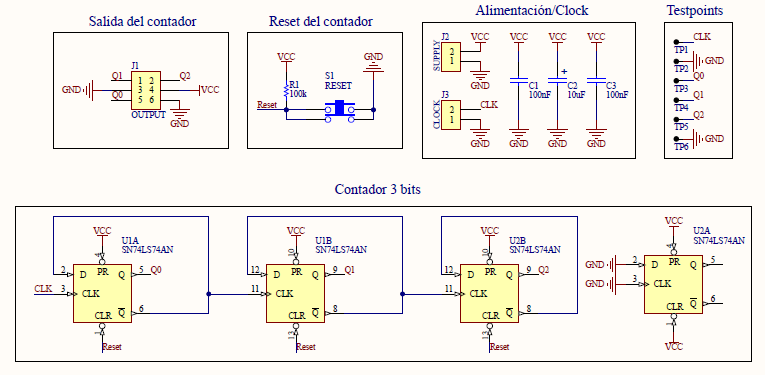
\includegraphics[scale=0.7]{../EJ7/Recursos/esquematico_asincronico.PNG}
    \caption{Esquem\'atico del PCB en Altium Designer}
    \label{fig:esquematico_asincronico}
\end{figure}

\begin{figure}[H]
    \centering
    \begin{tabular}{c c}
        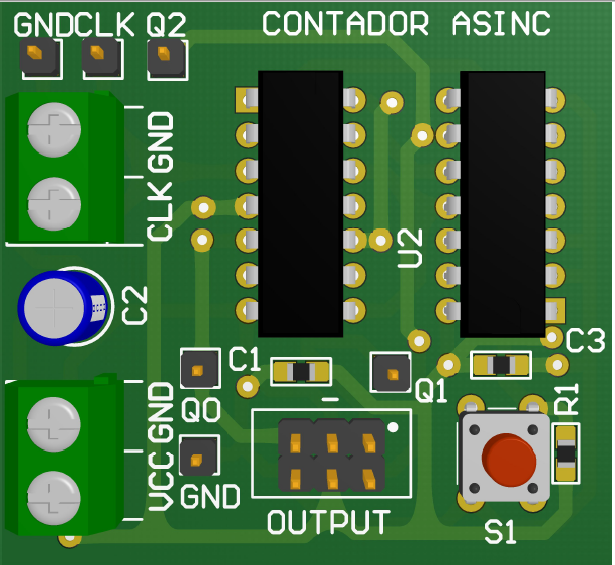
\includegraphics[scale=0.4]{../EJ7/Recursos/3d_top_asincronico.PNG} &
        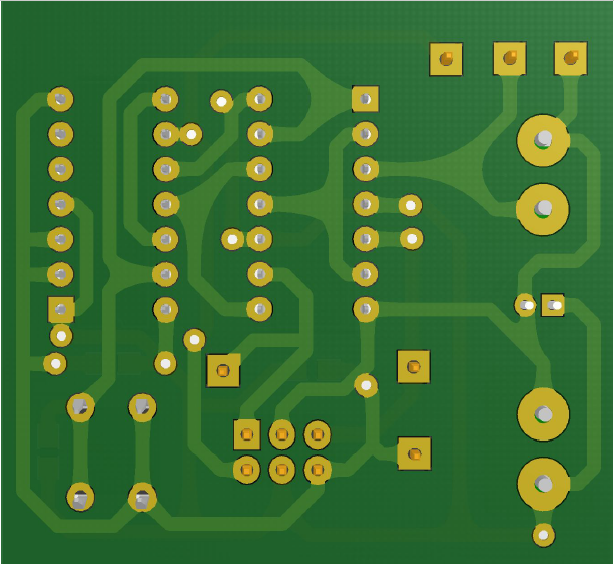
\includegraphics[scale=0.4]{../EJ7/Recursos/3d_bottom_asincronico.PNG} 
    \end{tabular}
    \caption{Dise\~no 3D del PCB}
    \label{fig:3d_asincronico}
\end{figure}

\subsection{Contador Sincr\'onico}
En esta secci\'on se propone el dise\~no de un contador sincr\'onico de 3 bits ascendente empleando \'unicamente Flip Flops D, por la misma raz\'on que para el caso asincr\'onico.
En un contador sincr\'onico, a diferencia del asincr\'onico, los proceso de cambio que ocurren en el mismo se dan sincronizados con respecto a un evento com\'un para lo cual es utilizada una se\~nal
de clock, cuyos flancos ascendentes producir\'an los cambios del contador de forma lo m\'as simult\'anea posible, ya que el evento llega de igual forma a todos y no hay una propagaci\'on como en el caso asincr\'onico.

\subsubsection{Dise\~no del circuito}
Para el circuito l\'ogico del contador se propone utilizar los flip flops como dispositivos que almacenen el estado de cada bit del contador,
luego utilizando l\'ogica externa se define c\'omo debe cambiar el estado ante un evento de sincronismo. Para ello se ilustra en la Tabla. \ref{table:tabla_verdad_contador}
la tabla de verdad del mismo. Entonces se pueden obtener las siguientes expresiones l\'ogicas:

\begin{equation}
    Q^{*}_0 = \neg Q_0 
\end{equation}

\begin{equation}
    Q^{*}_1 = Q_1 \oplus Q_0 
\end{equation}

\begin{equation}
    Q^{*}_2 = Q_2 \oplus (Q_1 \cdot Q_0) 
\end{equation}

\begin{table}[H]
    \centering
    \begin{tabular}{c c c | c c c}
        $Q_2$ & $Q_1$ & $Q_0$ & $Q^{*}_2$ & $Q^{*}_1$ & $Q^{*}_0$ \\ 
        \hline \\
        $0$ & $0$ & $0$ & $0$ & $0$ & $1$ \\
        $0$ & $0$ & $1$ & $0$ & $1$ & $0$ \\
        $0$ & $1$ & $0$ & $0$ & $1$ & $1$ \\
        $0$ & $1$ & $1$ & $1$ & $0$ & $0$ \\
        $1$ & $0$ & $0$ & $1$ & $0$ & $1$ \\
        $1$ & $0$ & $1$ & $1$ & $1$ & $0$ \\
        $1$ & $1$ & $0$ & $1$ & $1$ & $1$ \\
        $1$ & $1$ & $1$ & $0$ & $0$ & $0$ \\
    \end{tabular}
    \caption{Tabla de verdad estados actuales y futuros del contador}
    \label{table:tabla_verdad_contador}
\end{table}

Finalmente, se puede observar la implementaci\'on de estas expresiones en el circuito l\'ogico de la Fig. \ref{fig:esquematico_sincronico}.

\begin{figure}[H]
    \centering
        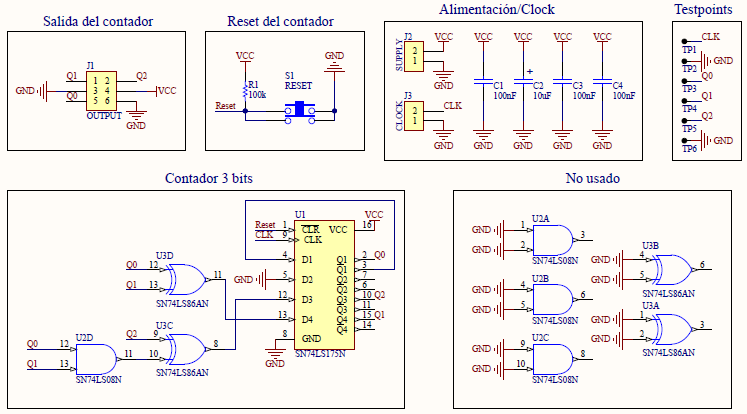
\includegraphics[scale=0.7]{../EJ7/Recursos/esquematico_sincronico.PNG}
    \caption{Esquem\'atico del PCB en Altium Designer}
    \label{fig:esquematico_sincronico}
\end{figure}

\begin{figure}[H]
    \centering
    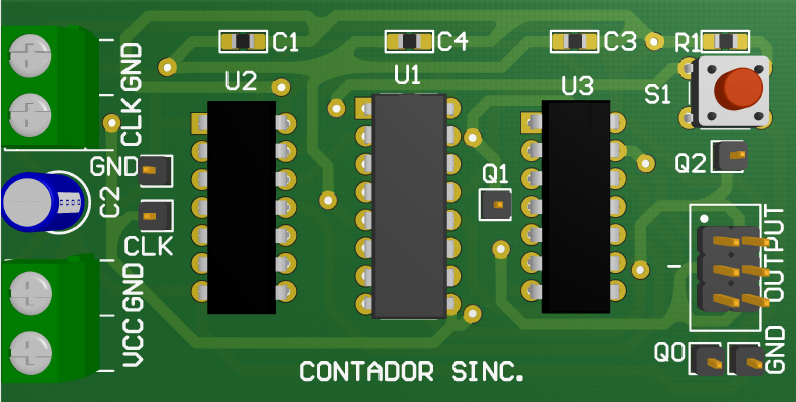
\includegraphics[scale=0.45]{../EJ7/Recursos/3d_top_sincronico.PNG}
    \caption{Dise\~no 3D del PCB}
    \label{fig:3d_sincronico_top}
\end{figure}

\begin{figure}[H]
    \centering
    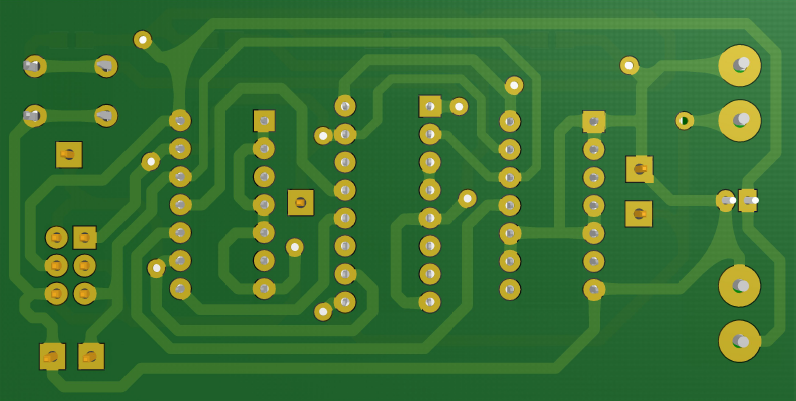
\includegraphics[scale=0.45]{../EJ7/Recursos/3d_bottom_sincronico.PNG} 
    \caption{Dise\~no 3D del PCB}
    \label{fig:3d_sincronico_bottom}
\end{figure}

\subsection{Visualizaci\'on del contador}
Se propone dise\~nar un circuito que decodifique el c\'odigo binario del contador y lo represente en un display
de 7 segmentos para poder realizar una prueba r\'apida del funcionamiento del circuito y poder visualizar el resultado del mismo.

\subsubsection{Dise\~no del circuito}
Se utilizar\'a un circuito integrado 74LS47, esto es, un decodificador BCD a 7 Segmentos, puesto que como la salida del contador se encuentra acotada
entonces puede ser interpretada como BCD. En este integrado la l\'ogica se encuentra negada, por lo cual es necesario utilizar un display de 7 segmentos de \'anodo com\'un,
donde el m\'aximo de corriente que puede soportar la salida del conversor es $25mA$, no obstante se har\'a circular una corriente de $4mA$ por segmento teniendo en cuenta que el modelo utilizado tiene una
tensi\'on $V_{D_ON} \approx 2.7V$.

Asumiendo el peor caso donde la tensi\'on sobre la resistencia es m\'axima y puede circular el m\'aximo de corriente, se limita al valor consignado y por ello se utilizan resistencias
de $R = \frac{5V - 2.7V}{4mA} > 575 \Omega \Rightarrow R = 680 \Omega$.

\begin{figure}[H]
    \centering
        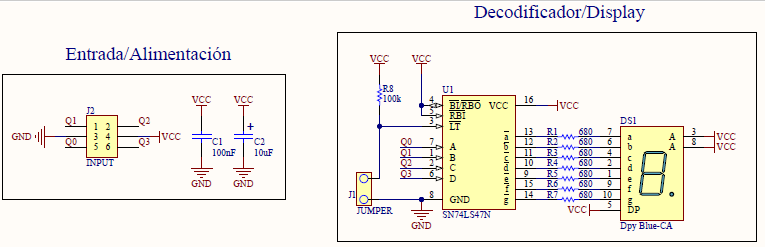
\includegraphics[scale=0.7]{../EJ7/Recursos/esquematico_visualizacion.PNG}
    \caption{Esquem\'atico del PCB en Altium Designer}
    \label{fig:esquematico_visualizacion}
\end{figure}

\begin{figure}[H]
    \centering
    \begin{tabular}{c c}
        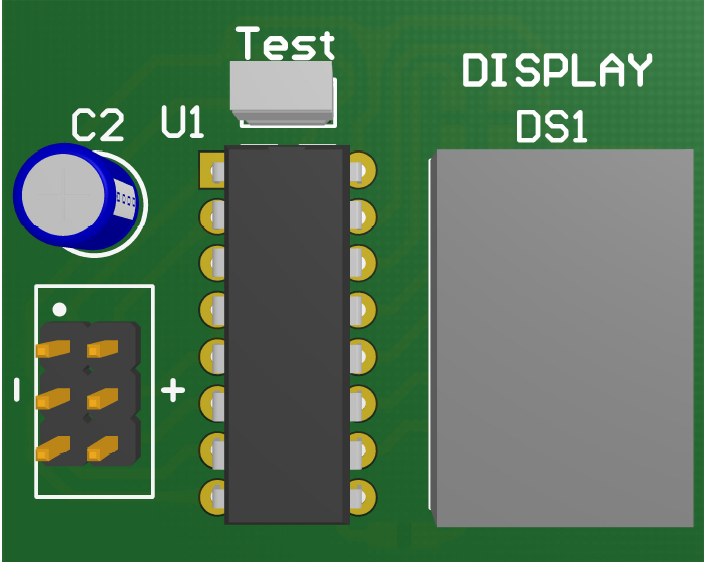
\includegraphics[scale=0.3]{../EJ7/Recursos/3d_top_visualizacion.PNG} &
        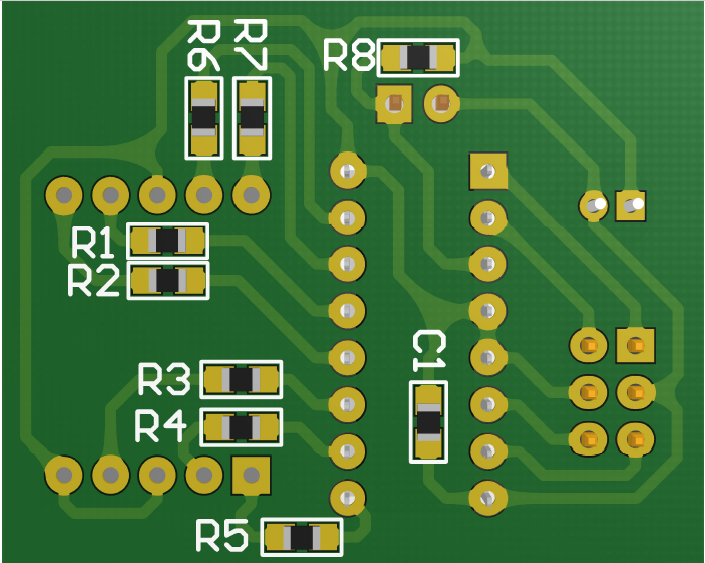
\includegraphics[scale=0.3]{../EJ7/Recursos/3d_bottom_visualizacion.PNG} 
    \end{tabular}
    \caption{Dise\~no 3D del PCB}
    \label{fig:3d_visualizacion}
\end{figure}

\subsection{Resultados}

\begin{figure}[H]
    \centering
        \begin{tabular}{c c}
            \includegraphics[scale=0.3]{../EJ7/Recursos/practica_0.jpeg} &
            \includegraphics[scale=0.3]{../EJ7/Recursos/practica_1.jpeg}
        \end{tabular}
    \caption{Implementaci\'on de ambos contadores, sincr\'onico y asincr\'onico}
    \label{fig:implementacion}
\end{figure}

\subsubsection{Mediciones}
Para ambos contadores, sincr\'onico y asincr\'onico, se mide por un lado la secuencia del mismo, utilizando los cuatro canales del osciloscopio
para poder observar en color amarillo la se\~nal de clock, la rosa corresponde al $Q_0$, la azul/violeta al $Q_1$ y luego la verde al $Q_2$. Por otro lado,
se mide el tiempo de propagaci\'on de los cambios de cada uno de los flip flops respecto del flanco del clock, para esta \'ultima medici\'on la referencia de colores se mantiene.

\begin{figure}[H]
    \centering
        \begin{tabular}{c c}
            \includegraphics[scale=0.2]{../EJ7/Mediciones/Osciloscopio/Segundo_Intento/Asincronico/cropped_contador.png} &
            \includegraphics[scale=0.2]{../EJ7/Mediciones/Osciloscopio/Segundo_Intento/Asincronico/cropped_salida_q0.png} \\
            \includegraphics[scale=0.2]{../EJ7/Mediciones/Osciloscopio/Segundo_Intento/Asincronico/cropped_salida_q1.png} &
            \includegraphics[scale=0.2]{../EJ7/Mediciones/Osciloscopio/Segundo_Intento/Asincronico/cropped_salida_q2.png}
        \end{tabular}
    \caption{Mediciones para Asincr\'onico entre punto medio y $V_{OH}$}
    \label{fig:asincronico_mediciones}
\end{figure}

\begin{figure}[H]
    \centering
        \begin{tabular}{c c}
            \includegraphics[scale=0.2]{../EJ7/Mediciones/Osciloscopio/Segundo_Intento/Sincronico/cropped_contador.png} &
            \includegraphics[scale=0.2]{../EJ7/Mediciones/Osciloscopio/Segundo_Intento/Sincronico/cropped_salida_q0.png} \\
            \includegraphics[scale=0.2]{../EJ7/Mediciones/Osciloscopio/Segundo_Intento/Sincronico/cropped_salida_q1.png} &
            \includegraphics[scale=0.2]{../EJ7/Mediciones/Osciloscopio/Segundo_Intento/Sincronico/cropped_salida_q2.png}
        \end{tabular}
    \caption{Mediciones para Sincr\'onico entre punto medio y $V_{OH}$}
    \label{fig:sincronico_mediciones}
\end{figure}

\subsubsection{An\'alisis de datos}
Resulta de inter\'es observar como anomal\'ia el hecho de que la salida de todos los flip flops no era de $5 V$ sino de $4 V$,
no obstante se encontraba dentro del margen de $V_{OH}$ seg\'un lo provisto por el fabricante. 

En la Fig. \ref{fig:asincronico_mediciones} se puede observar como la forma en que el clock de cada bit depende del anterior en peso produce una propagaci\'on de los tiempos, con lo cual ello explica
la raz\'on de que en esa medida los tiempos hayan ido incrementando bit a bit en el contador. Es por esto que el tiempo de propagaci\'on total
del contador es de $t_p = 55.5nS$, con lo cual cualquier frecuencia de clock que quiera producir un cambio en menos tiempo de esto va a ser ignorada, por ende, limita la frecuencia de operaci\'on a
$f_{MAX} = 18.01MHz$.

En el caso de las mediciones de la Fig. \ref{fig:sincronico_mediciones}, para determinar la frecuencia
m\'axima de operaci\'on es necesario tener en cuenta la respuesta m\'as lenta, es decir, $t_p = 25.6nS \Rightarrow f_{MAX} = 39.03MHz$.

\begin{table}[H]
    \centering
    \begin{tabular}{c c}
        \hline \\
        Contador Asincr\'onico & $f_{MAX} = 18.01MHz$ \\
        Contador Sincr\'onico & $f_{MAX} = 39.03MHz$ \\
        \hline
    \end{tabular}
\end{table}

\subsection{Conclusi\'on}
En conclusi\'on, los procesos sincr\'onicos ser\'an siempre o en la mayor\'ia de los casos m\'as r\'paidos que los proceso asincr\'onicos,
desde el punto de vista en el cual, con un enfoque sincr\'onico se garatiza que los mecanisco involucrados en el funcionamiento de dicho proceso
sean ejecutados o puestos en marcha de forma casi simult\'anea. No sucede as\'i en los procesos asincr\'onicos, como en este contador, donde haya 
una dependencia de tales mecanismos que produzca una propagaci\'on de tiempos que se incrementen.
	\newpage
	\section{Ejercicio 8: Dise\~no de controlador para un Joystick Anal\'ogico}

\end{document}
